\chapter{The role of the stratosphere in seasonal prediction}

\section{Introduction}

Accurate prediction of the atmospheric circulation several months in advance
relies on the presence of low-frequency predictable signals in the climate
system. It has now been demonstrated that the stratosphere is an important
pathway for the communication of predictable tropical signals across the globe;
in particular, the El Ni\~no-Southern Oscillation (ENSO) \citep{Pascoe2006,
Bell2009, Ineson2009, Hurwitz2011}, Quasi-Biennial Oscillation (QBO)
\citep{Marshall2009, Garfinkel2011}, and 11-year solar cycle \citep{Kodera2002,
Gray2013}. These teleconnections allow for the possibility of significant
predictability in regions remote from the direct effect of the signal. Despite
this, many operational seasonal forecast models include only a poor
representation of the stratosphere \citep{Maycock2011}, and it has been
suggested that this contributes to their lack of seasonal forecast skill in the
extratropics \citep{Smith2012}.

Furthermore, because stratospheric anomalies persist for longer than those in
the troposphere and can influence surface weather patterns
\citep[e.g.,][]{Baldwin2001a}, the initial conditions of the stratosphere itself
can act as a source of enhanced predictability \citep{Baldwin2003a,
Charlton2003, Hardiman2011}. The effect of the stratosphere on the troposphere
is most pronounced following a rapid midwinter breakdown of the strong westerly
stratospheric polar vortex (known as a stratospheric sudden warming, SSW), and
past work has focused on the influence of these events on forecast skill
\citep{Kuroda2008, Sigmond2013}. However, SSWs are highly nonlinear events which
are currently not predictable beyond about two weeks in advance
\citep{Marshall2010}, limiting their usefulness in seasonal prediction. SSWs
also occur almost exclusively in the Northern Hemisphere (NH), with only one
event in the approximately 60 year record having been observed in the Southern
Hemisphere (SH), in September 2002 \citep{Roscoe2005}. 

The rarity of SSWs in the SH is a result of less dynamical forcing from
vertically propagating planetary waves in the SH relative to the NH
stratosphere. This, in turn, comes about because of lesser SH orography and
land-sea temperature contrasts which can excite planetary waves. This reduced
variability also means that anomalies in the Antarctic stratosphere persist for
longer than those in the Arctic \citep{Simpson2011}, so they may be predictable
on longer time scales, and so more useful for seasonal forecasts, despite the
lack of SSWs. Indeed, \citet{Thompson2005} and \citet{Son2013a} have found that
smaller-amplitude variations in the Antarctic stratospheric polar vortex are
followed by coherent temperature and pressure anomalies at the Earth's surface
which resemble the Southern Annular Mode (SAM) pattern. These observations led
\citet{Roff2011} to find that improved forecasts of the SAM up to 30 days ahead
may be achieved with a stratosphere-resolving model. The SAM is the dominant
mode of variability of the extratropical Southern Hemisphere and affects the
position of storm tracks, rainfall, surface air temperature, and ocean
temperatures across the extratropics \citep[e.g.,][]{Silvestri2003, Reason2005,
Hendon2007}. As such, there are considerable societal benefits, and interests in
its prediction \citep{Lim2013}.

Another reason for interest in the prediction of the Antarctic stratosphere is
the interannual variability in springtime ozone depletion. The magnitude of this
interannual variability is a significant fraction of the magnitude of long-term
depletion caused by emission of chlorofluorocarbons (CFCs) and other
ozone-depleting substances. While ozone-depleted air is confined over the polar
region by the stratospheric polar vortex during winter and spring (resulting in
the ozone hole), following the ultimate breakdown of the vortex (final warming)
in late spring/early summer, this air becomes released to mid-latitudes. The
extent of this summertime ozone depletion is largely determined by the total
deficit in ozone over the Antarctic during spring
\citep{Bodeker2005}. Interannual variability in springtime ozone depletion can
therefore significantly affect the amount of harmful ultraviolet radiation
reaching the Earth's surface over more populated areas of the Southern
Hemisphere.

\citet{Salby2012} have shown that interannual variations in Antarctic ozone
depletion are highly correlated with changes in planetary wave forcing of the
stratosphere. They found that the anomalous vertical Eliassen-Palm (EP) flux (a
measure of the momentum transmitted by planetary waves) entering the
stratosphere poleward of 40$^{\circ}$S during August-September explains almost
all the interannual variance of anomalous ozone depletion during
September--November. Using this relationship, they postulate that accurate
prediction of planetary wave forcing could allow skillful seasonal forecasts of
ozone depletion.

The influence of planetary wave forcing on ozone depletion comes about through
both chemical and dynamical mechanisms. Planetary wave breaking causes an
increase of the strength of the stratospheric residual mean meridional
circulation \citep{Haynes1991}, with a resultant increase in large-scale descent
and adiabatic warming over the pole. This warming inhibits the formation of
polar stratospheric clouds which have a vital role in the activation of halogen
species that cause the chemical depletion of ozone. The increased meridional
circulation as well as an enhancement of horizontal two-way mixing caused by
planetary wave breaking, also cause an increase in the dynamical transport of
tropical ozone-rich air to the polar regions, further increasing ozone
concentrations.  Breaking planetary waves can also modify the geometry of the
stratospheric polar vortex, stripping away elements of ozone-depleted air
\citep{Waugh1994}, or in the extreme case of the 2002 SSW cause the ozone hole
to split in two \citep{Charlton2005a}.

Here, we address directly the influence of the stratosphere on springtime
Antarctic seasonal forecast skill using a set of historical hindcasts (or
historical re-forecasts) of a new operational system with a fully
stratosphere-resolving general circulation model. We find significant skill in
the prediction of the Antarctic stratospheric polar vortex up to four months in
advance, and even of the 2002 SSW. Using the observed relationship between
column ozone quantities and the stratospheric circulation, we are then able to
infer skillful predictions of springtime ozone depletion, confirming the
hypothesis of \citet{Salby2012}. This exceeds the lead-time of other
contemporary ozone forecasts, which are typically no more than two weeks (Eskes
2005). The forecast system also shows highly significant levels of skill in the
prediction of the surface SAM at seasonal lead times. By studying the variation
of hindcast skill with time and height, we demonstrate that this skill is
significantly influenced by the descent of long-lived stratospheric circulation
anomalies.




\section{Seasonal forecast system}

The analysis in this paper is based on results from a set of hindcast
predictions produced by the Met Office Global Seasonal Forecast System 5
(GloSea5) \citep{MacLachlan2014}. This system is based upon the HadGEM3 coupled
general circulation model \citep{Hewitt2011}, with an atmospheric resolution of
0.83$^{\circ}$ longitude by 0.56$^{\circ}$ latitude, 85 quasi-horizontal
atmospheric levels and an upper boundary at 85~km. The ocean resolution is
0.25$^{\circ}$ in longitude and latitude, with 75 quasi-horizontal levels. A
15-member ensemble of hindcasts was run for each year in the period
1996--2009. The hindcast length is approximately four months from three separate
start dates spaced two weeks apart and centered on 1st August (07/25, 08/01,
08/09), with 5 members initialised on each start date. Members initialised on
the same start date differ only by stochastic parameterization of model physics
\citep{Tennant2011}.

Initial conditions for the atmosphere and land surface were taken from the
ERA-Interim reanalysis \citep{Dee2011}, and initial ocean and sea-ice
concentrations from the GloSea5 Ocean and Sea Ice Analysis, based on the FOAM
data assimilation system \citep{Blockley2013}. Beyond initialisation the model
takes no further observational data, and contains no flux corrections or
relaxations to climatology. The model lacks interactive chemistry, and ozone
concentrations are fixed to observed climatological values averaged over
1994--2005, including a seasonal cycle \citep{Cionni2011}.

\citet{Scaife2013} have shown that this seasonal forecast system produces
unprecedented skillful forecasts of the North Atlantic Oscillation during the
Northern Hemisphere winter. The combined effects of ENSO, QBO and sea-ice
teleconnections, as well as to the increased ocean resolution, which has
improved the representation of Northern Hemisphere blocking events
\citep{Scaife2011a} contribute to this skill.

Hindcast accuracy is verified by comparison to the ERA-Interim reanalysis
\citep{Dee2011}. This provides a `clean comparison' since the hindcasts exactly
match ERA-Interim at the initialisation date. The ERA-Interim data set has been
demonstrated to have realistic representation of the stratospheric meridional
circulation \citep{Seviour2012, Monge-Sanz2013}. It also assimilates
observations of ozone concentrations, and this assimilation has been
demonstrated to be in close agreement with independent satellite data
\citep{Dragani2011}.

\section{Northern Hemisphere results}

% NH data
% 8.5 events/decade - 3.5 splits, 5.0 displs 
% min 47% (01/02) max 100% (97/98) (any event in winter)

\begin{figure}[t]
  \noindent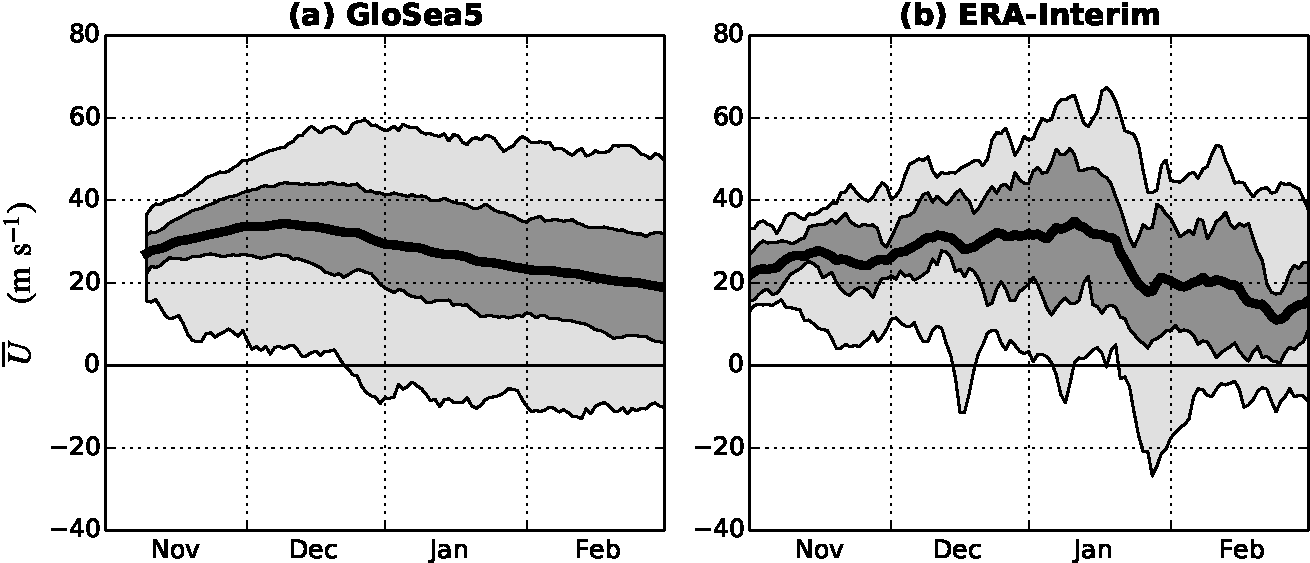
\includegraphics[width=\textwidth,angle=0]{figures/chapter-seasonal/zmzw_climatologies_nh.pdf}\\
  \caption[Comparison of GloSea5 and ERA-Interim zonal-mean zonal wind
climatologies.]{Time series of daily 10~hPa zonal-mean zonal wind
($\overline{U}$) at 60$^{\circ}$S for all GloSea5 ensemble members from
1996--2009 (a) and ERA-Interim from 1979--2010 (b). The thick black line
indicates the mean, dark grey shading the interquartile range and light grey the
95th percentile range. Individual time series of the two ensemble members of
GloSea5 which simulate an SSW (one for 1997 and one for 2002), and the year with
an observed SSW (2002) are shown in red.}\label{fig:sh_zmzw_clim}
\end{figure}

\begin{figure}[t] \centering
  \noindent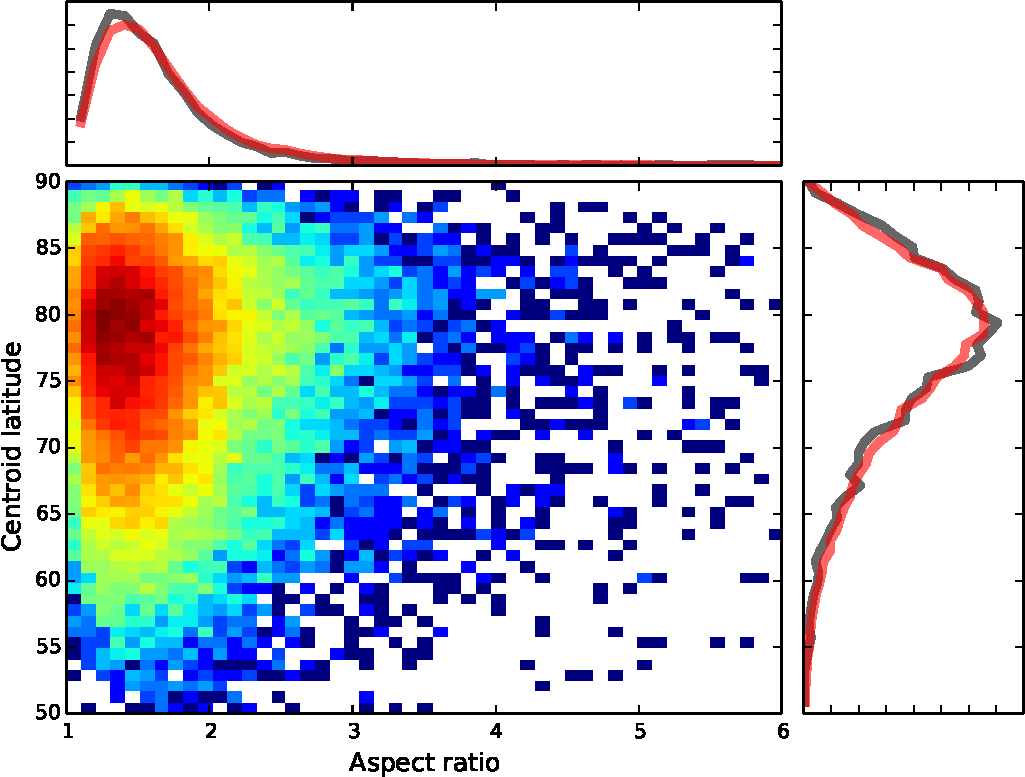
\includegraphics[width=0.7\textwidth,angle=0]{figures/chapter-seasonal/GloSea_moments_histogram.pdf}\\
  \caption[]{}\label{fig:sh_zmzw_clim}
\end{figure}


\begin{figure}[t]
  \noindent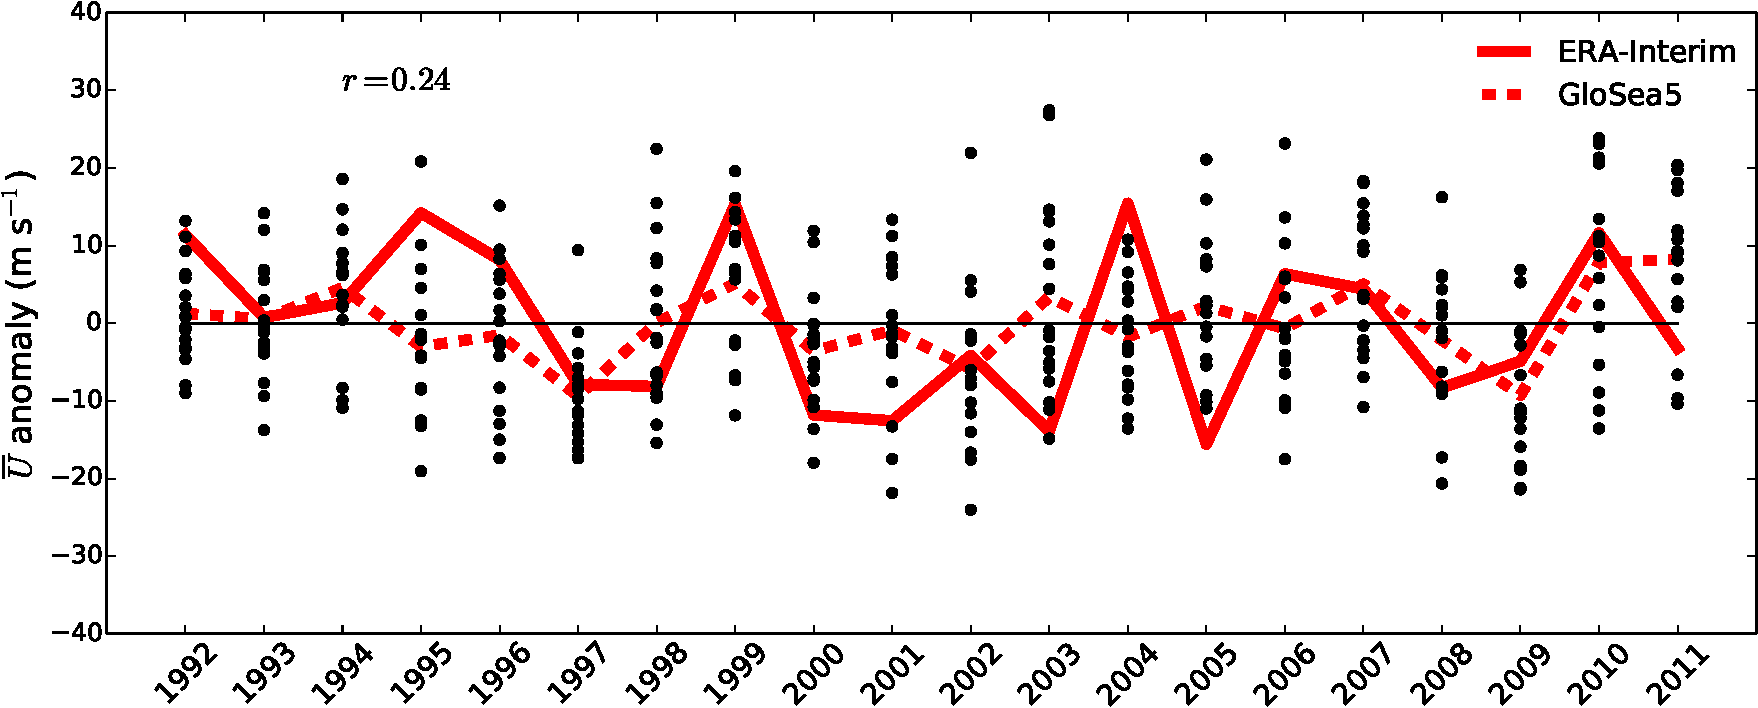
\includegraphics[width=\textwidth,angle=0]{figures/chapter-seasonal/DJF_ZMZW_NH.pdf}\\
  \caption[]{}\label{fig:sh_zmzw_clim}
\end{figure}


\begin{figure}[t] \centering
  \noindent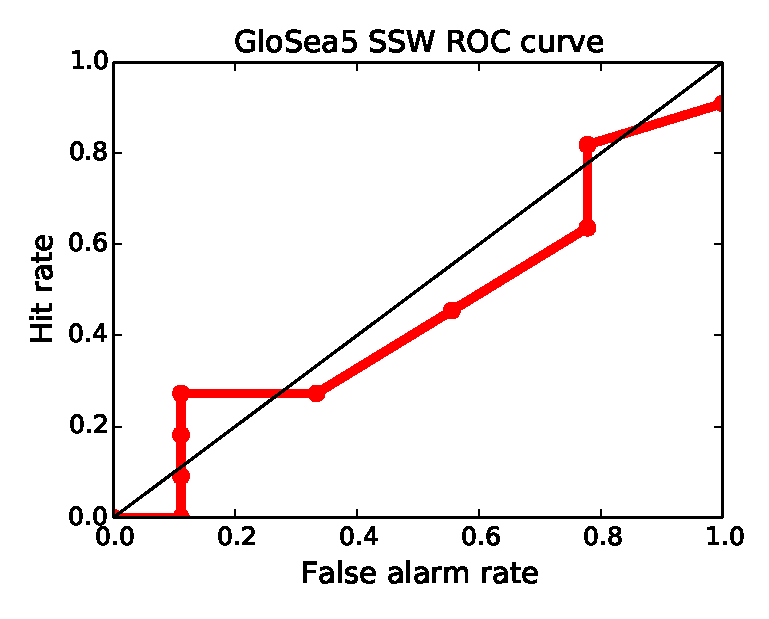
\includegraphics[width=0.7\textwidth,angle=0]{figures/chapter-seasonal/SSW_ROC.pdf}\\
  \caption[]{}\label{fig:sh_zmzw_clim}
\end{figure}

\begin{figure}[t] \centering
  \noindent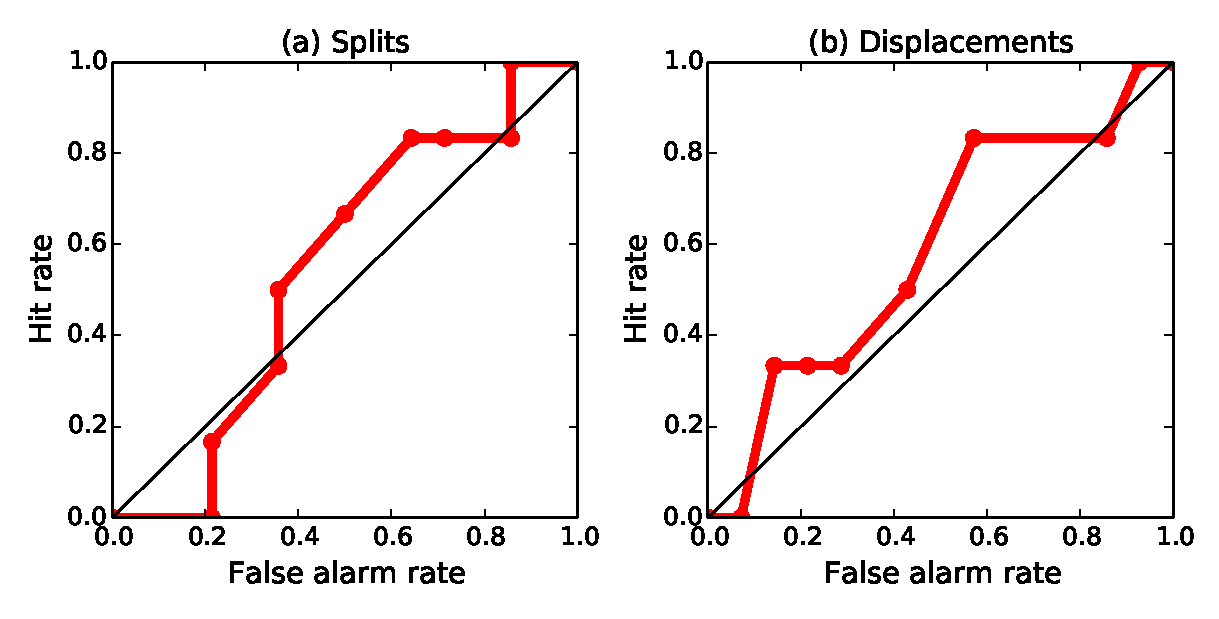
\includegraphics[width=\textwidth,angle=0]{figures/chapter-seasonal/glosea_split_displ_ROC_any.pdf}\\
  \caption[]{}\label{fig:sh_zmzw_clim}
\end{figure}

\begin{figure}[t] \centering
  \noindent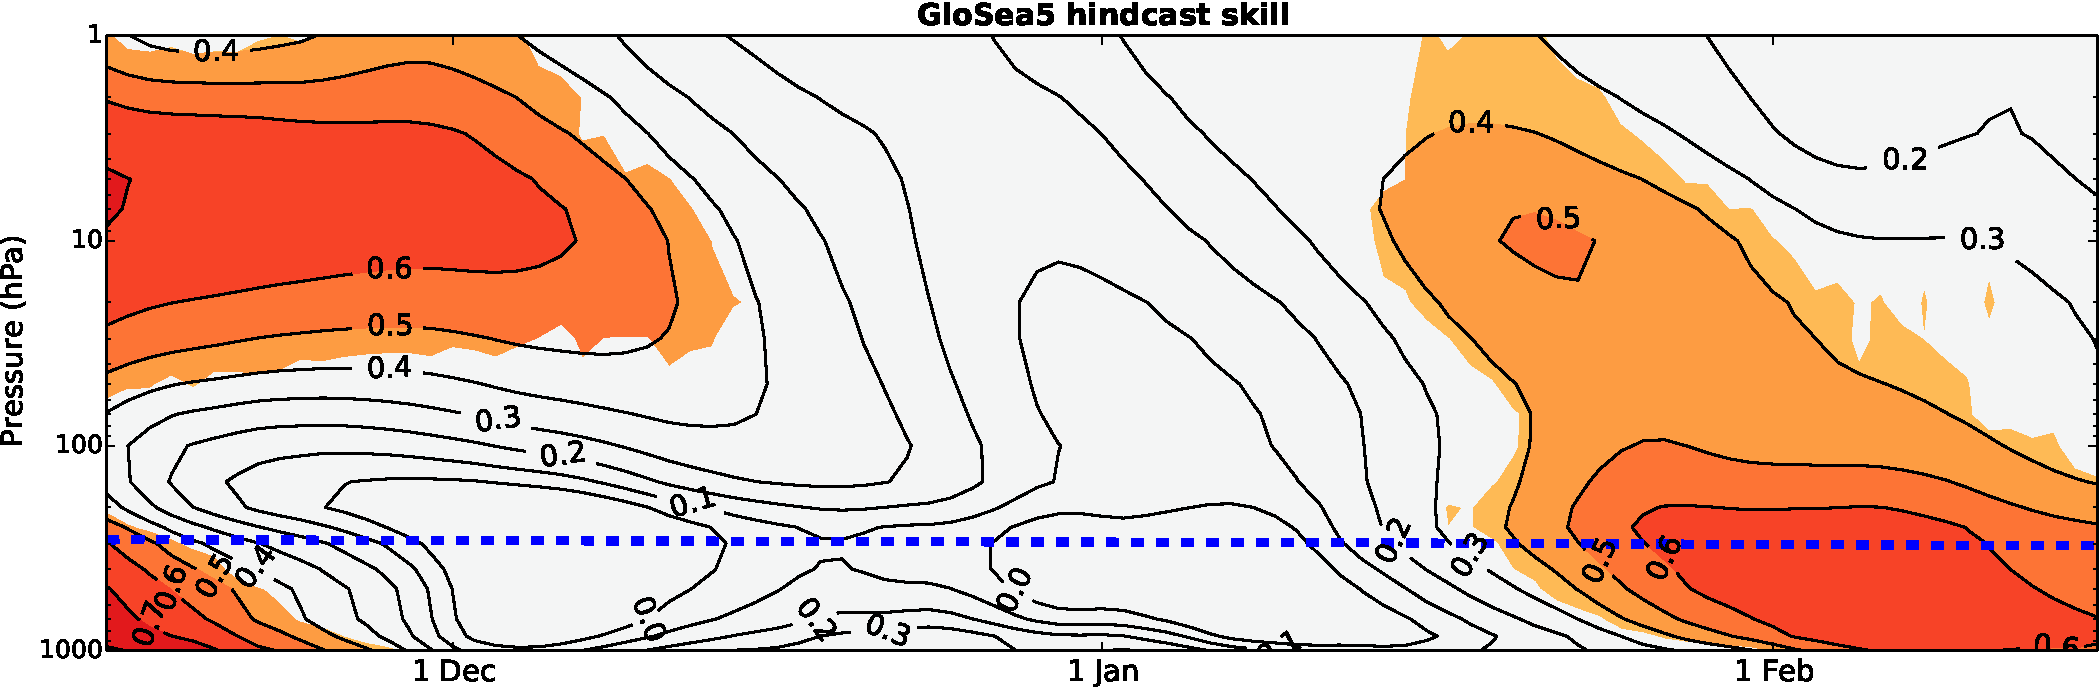
\includegraphics[width=\textwidth,angle=0]{figures/chapter-seasonal/NH_lag_height_corr.pdf}\\
  \caption[]{}\label{fig:sh_zmzw_clim}
\end{figure}




\section{Southern Hemisphere results}


\subsection{Stratospheric polar vortex}

The climatology of Antarctic stratospheric polar vortex winds in the GloSea5
hindcasts is compared to the ERA-Interim reanalysis climatology in Fig.\
\ref{fig:sh_zmzw_clim}. The strength of the stratospheric polar vortex is
measured by the zonal-mean zonal wind ($\overline{U}$) at 60$^{\circ}$S and
10~hPa, which is approximately the center of the mean position of the vortex in
the mid-stratosphere. The composite for the GloSea5 hindcasts is formed from all
the individual ensemble members over 1996--2009 (a total of 210 realizations),
while that from ERA-Interim is a composite of all years from 1979--2010 (a total
of 32 years). It can be seen that the mean of the GloSea5 hindcasts agrees very
closely with ERA-Interim throughout the spring, with only a slight bias towards
weaker winds in August and September. The interquartile and 95th percentile
ranges of GloSea5 and ERA-Interim also agree well, although the ERA-Interim
values are noisier as would be expected from a sample size consisting of fewer
years.

\begin{figure}[t]
  \noindent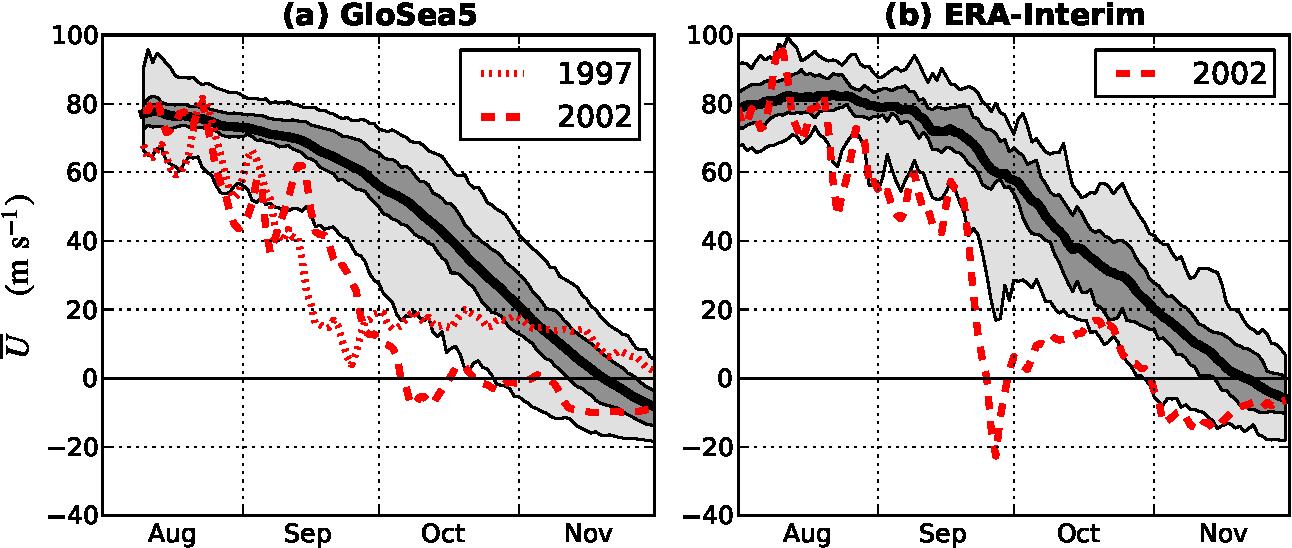
\includegraphics[width=\textwidth,angle=0]{figures/chapter-seasonal/zmzw_climatologies_crop.pdf}\\
  \caption[Comparison of GloSea5 and ERA-Interim zonal-mean zonal wind
climatologies.]{Time series of daily 10~hPa zonal-mean zonal wind
($\overline{U}$) at 60$^{\circ}$S for all GloSea5 ensemble members from
1996--2009 (a) and ERA-Interim from 1979--2010 (b). The thick black line
indicates the mean, dark grey shading the interquartile range and light grey the
95th percentile range. Individual time series of the two ensemble members of
GloSea5 which simulate an SSW (one for 1997 and one for 2002), and the year with
an observed SSW (2002) are shown in red.}\label{fig:sh_zmzw_clim}
\end{figure}

The GloSea5 hindcast skill for the prediction of the Antarctic stratospheric
polar vortex winds is shown in Fig.\ \ref{fig:zmzw_ozone}(a). Anomalies are
defined from the relevant climatology of either GloSea5 or ERA-Interim. For
GloSea5, this climatology is calculated from the mean of each day across all
ensemble members in all years, while for ERA-Interim the climatology is the mean
of each day, smoothed with a 30-day running mean (in order to account for its
increased noise due to the fact it consists of only a single
realization). Results are shown for September--November (SON) averages,
corresponding to a 1--4 month lead time. The correlation between the GloSea5
ensemble mean and ERA-Interim is 0.73, which is statistically significant at the
99\% confidence level. This correlation does not depend strongly on particular
years; the correlation remains significant at the 95\% level ($r=0.57$) if the
year 2002 is excluded. Significance is calculated using a two-tailed bootstrap
test, whereby the percentile of the observed correlation is calculated from a
distribution formed by the correlation of a large number ($\sim 10,000$) of
pairs of time series formed by re-sampling with replacement from the original
time series. These significance tests make fewer assumptions about the
underlying structure of the data than parametric tests \citep{Wilks}, and are
used throughout this study.

\begin{figure}[t]
  \noindent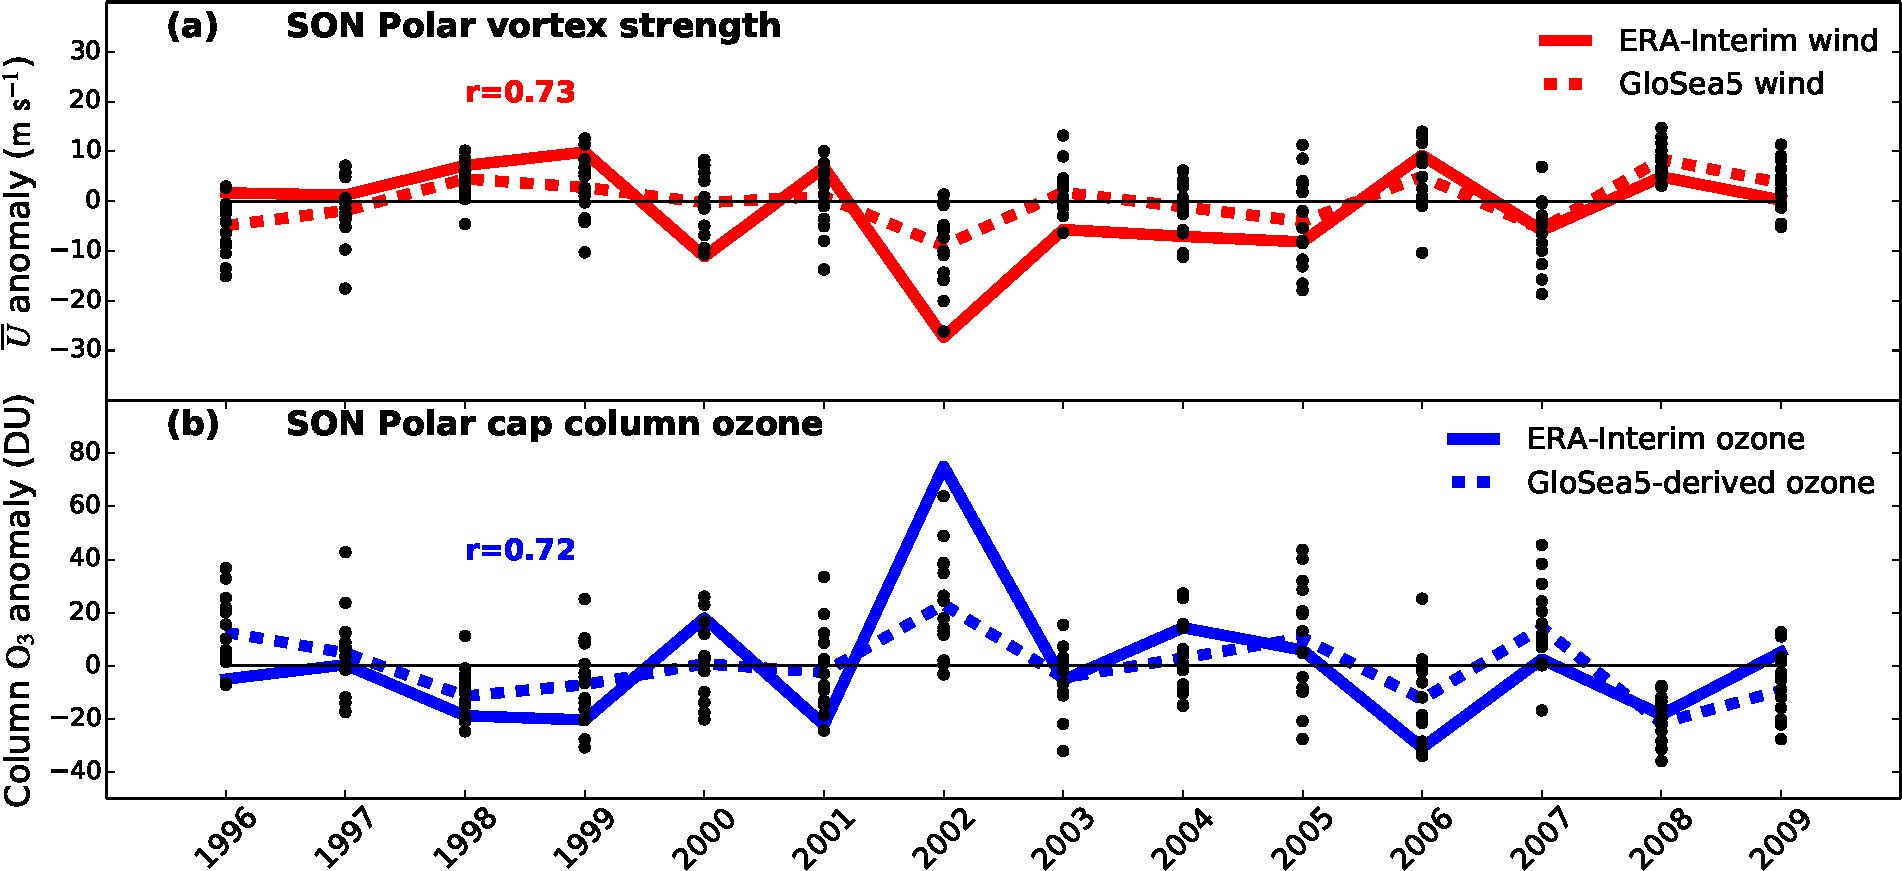
\includegraphics[width=\textwidth,angle=0]{figures/chapter-seasonal/zmzw_ozone_crop.pdf}\\
  \caption[GloSea5 forecast skill for the stratospheric polar vortex strength
and column ozone.]{(a) SON mean anomalies at 10~hPa and 60$^{\circ}$S in
ERA-Interim and the GloSea5 hindcast ensemble mean. (b) SON mean polar cap
averaged (60--90$^{\circ}$S) total column ozone anomalies from ERA-Interim and
those derived from the GloSea5 anomalies as described in the text. Individual
ensemble members are shown as black dots. Hindcasts are initialised near 1st
August.}\label{fig:zmzw_ozone}
\end{figure}

Two SSW events were simulated in the GloSea5 hindcasts; in 1997 and 2002. Time
series of stratospheric polar vortex winds for these events are shown in Fig.\
\ref{fig:sh_zmzw_clim}(a) along with the observed 2002 SSW in Fig.\
\ref{fig:sh_zmzw_clim}(b). Note that although $\overline{U}$ at 60$^{\circ}$S
and 10~hPa does not quite become easterly for the 1997 event, it does become
easterly \emph{poleward} of 60$^{\circ}$S, which satisfies the World
Meteorological Organization definition of a SSW. Given the total of 210 ensemble
hindcasts, these two simulated events suggest a frequency of Southern Hemisphere
SSW events of approximately one in 100 years in the current climate (making the
assumption that the model can accurately simulate the probability of these
events). It can also be seen that 2002 has the most anomalous stratospheric
polar vortex in the GloSea5 hindcasts, with 14 of 15 ensemble members simulating
negative anomalies, and the most negative ensemble mean. It is therefore
possible that the 2002 event was to some degree predictable about two months in
advance, although it has not been determined whether this predictability comes
from a preconditioning of the vortex, as suggested by \citet{Scaife2005c}, or
the result of external forcing.

It should be noted that both the SSW events simulated by GloSea5 were vortex
displacement events, in contrast to the vortex splitting event which occurred in
2002 \citep{Charlton2005a}. This is demonstrated in Fig.\ \ref{fig:sh_ssws}, which
shows geopotential height in the mid-stratosphere at the central date (date of
minimum at $\overline{U}$ 60$^{\circ}$S and 10~hPa) of the two simulated events
in GloSea5 and the observed event in ERA-Interim. The distinction between
splitting and displacement SSW events is important because it has been observed
that tropospheric anomalies are greater following vortex splitting events, at
least in the Northern Hemisphere \citep{Nakagawa2006, Mitchell2013}.

\begin{figure}[t]
  \noindent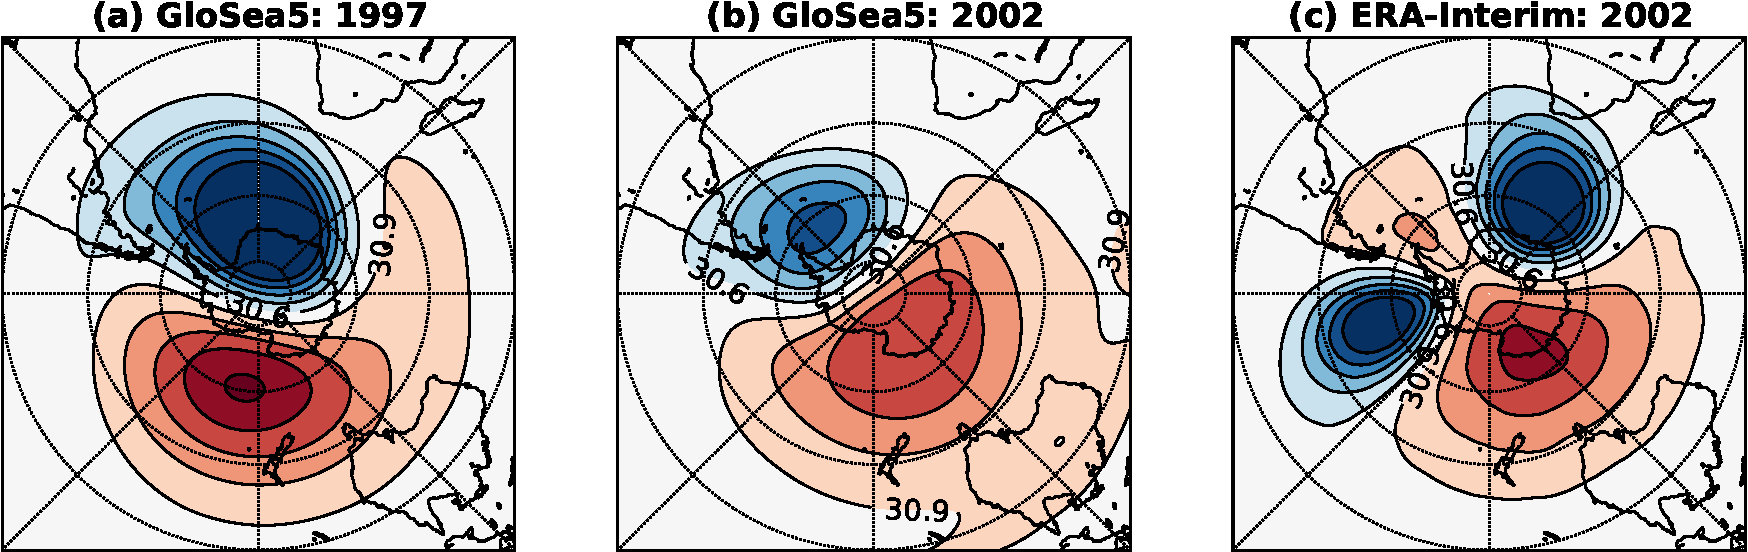
\includegraphics[width=\textwidth,angle=0]{figures/chapter-seasonal/ssws_crop.pdf}\\
  \caption[Comparison of GloSea5 and observed SSWs.]{Geopotential height at
10~hPa at the central date (date at which $\overline{U}$ at 60$^{\circ}$S,
10~hPa is at its minimum value) of the two GloSea5 ensemble members which
simulate a SSW (a,b), and for ERA-Interim at the central date of the 2002 SSW
(c). Units are km and the contour interval is 0.3~km.}\label{fig:sh_ssws}
\end{figure}


The timing of the final warming of the stratospheric polar vortex has a
significant effect on stratospheric temperature and ozone concentrations
\citep{Yamazaki1987}, as well as coupling of the stratosphere to the troposphere
\citep{Black2007}. The predictability of these events was investigated in
GloSea5, but not found to be highly significant. This is probably because the
mean timing of the final warming is towards the end of the four month hindcast
simulation (around 20th November at 10~hPa), and the final warming does not
occur before the end of the hindcast for some ensemble members, thereby
introducing a bias in the mean. It is likely that shorter lead-time forecasts
would be required to produce skillful predictions of the final warming date.


\subsection{Ozone depletion}

GloSea5 does not include interactive ozone chemistry, so in order to make ozone
forecasts concentrations must be inferred from other meteorological
variables. Total ozone quantities over the Antarctic polar cap have been found
to be highly correlated with vertical EP flux poleward of 40$^{\circ}$S
\citep{Weber2011, Salby2012}. This diagnostic is not likely to be produced
directly by operational seasonal forecast systems and requires high frequency
output at high spatial resolution to calculate. However, vertical EP flux
dominates variability of the stratospheric polar vortex, so it may be possible
to use the strength of the vortex to infer ozone quantities.

SON mean total column ozone quantities area-weighted averaged over the polar cap
(60--90$^{\circ}$S) are shown in Fig.\ \ref{fig:zmzw_scatter}(a) for ERA-Interim
and the Total Ozone Mapping Spectrometer (TOMS) satellite instrument
\citep{Kroon2008}. ERA-Interim data are highly correlated with TOMS, verifying
the accuracy of ERA-Interim against direct satellite measurements (TOMS values
are slightly higher than ERA-Interim; this is probably because TOMS cannot make
observations during the polar night). The long-term trend in polar cap total
column ozone is calculated by fitting a second-order polynomial to the
data. This long-term trend is due to changes in concentrations of CFCs and other
ozone-depleting substances, and largely unrelated to dynamical variability. On
the other hand, shorter-term interannual changes are strongly related to
dynamical variability. In Fig.\ \ref{fig:zmzw_scatter}(b) anomalies of polar cap
total column ozone from the long-term trend are plotted against anomalies of the
SON mean $\overline{U}$ at 60$^{\circ}$S and 10~hPa. It can be seen that these
two quantities are highly correlated ($r=-0.92$), meaning polar vortex
variability explains approximately 85\% of the variance of polar cap total
column ozone anomalies.

\begin{figure}[t]
  \noindent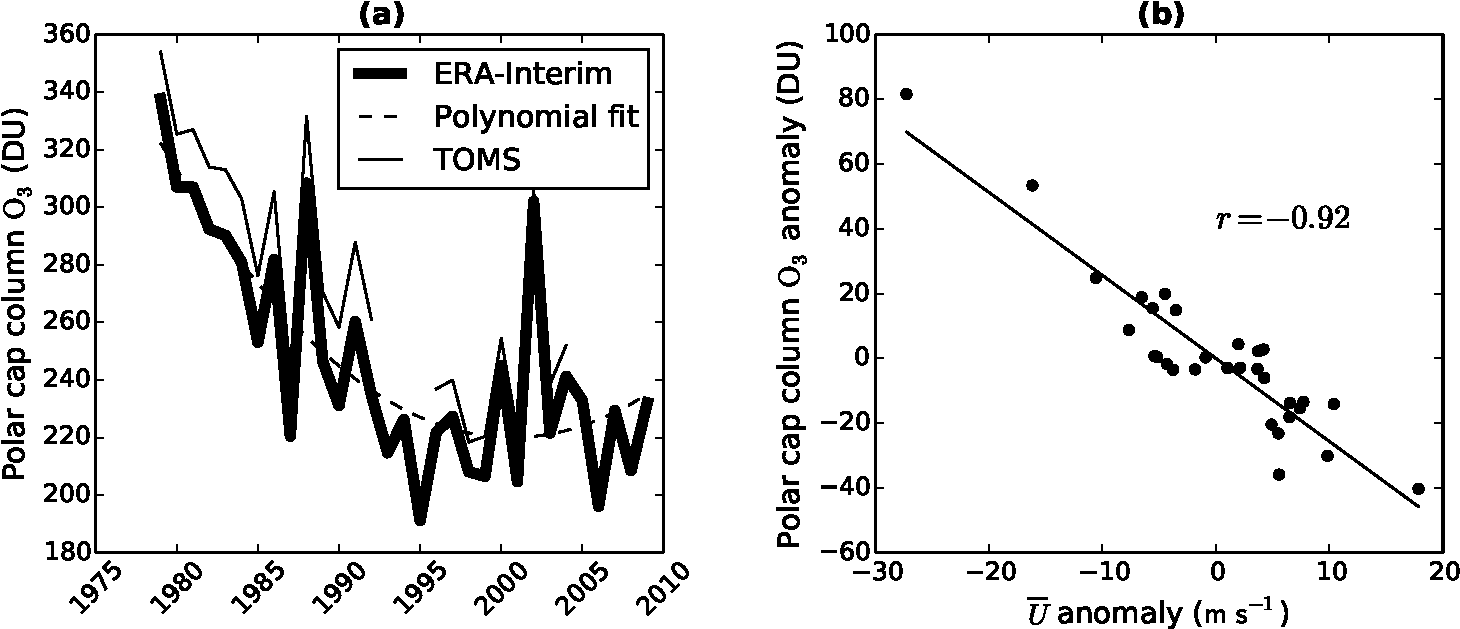
\includegraphics[width=\textwidth,angle=0]{figures/chapter-seasonal/zmzw_ozone_scatter_crop.pdf}\\
  \caption[Relation between stratospheric polar vortex strenth and column
ozone.]{(a) Time series of SON mean polar cap averaged (60-90$^{\circ}$S) total
column ozone in ERA-Interim and the TOMS satellite instrument. The ERA-Interim
data are fitted with a 2nd-order polynomial. (b) Anomalies of ERA-Interim column
ozone from the polynomial fit plotted against SON mean anomalies at 10~hPa and
60$^{\circ}$S for each year from 1979--2009.} \label{fig:zmzw_scatter}
\end{figure}

This observed correlation can be used with the GloSea5 forecasts of polar vortex
winds to produce inferred predictions of polar cap total column ozone
quantities. Figure \ref{fig:zmzw_ozone}(b) shows the GloSea5 hindcasts along
with the assimilated values from ERA-Interim. The correlation between the
GloSea5 ensemble mean and ERA-Interim is 0.72, which is statistically
significant at the 99\% level. Errors from the regression in Fig.\
\ref{fig:zmzw_ozone}(b) for the inferred ozone quantities for each ensemble
member are small compared to the spread between ensemble members, and so not
plotted in this figure.

\subsection{Southern Annular Mode}

The SAM index in both GloSea5 and ERA-Interim is depicted as the difference
between the normalized anomalies of zonally averaged mean sea-level pressure at
40$^{\circ}$S and 65$^{\circ}$S \citep{Gong1999}. These anomalies are calculated
from the respective climatologies of GloSea5 and ERA-Interim. The ERA-Interim
SAM index calculated in this way is also highly correlated with other measures
of the SAM, such as the station-based index of \citet{Marshall2003}. The GloSea5
hindcast skill for the prediction of the seasonal (SON) mean SAM index is shown
in Fig.\ \ref{fig:sam_ts}. The correlation of the GloSea5 ensemble mean and
ERA-Interim is 0.64, which is statistically significant at the 99\% level,
confirming skillful prediction of the SAM at 1--4 month lead times. This is
similar to the value for the NAO correlation skill of 0.62 found by
\citet{Scaife2013} in the same seasonal forecast system.

\begin{figure}[t]
  \noindent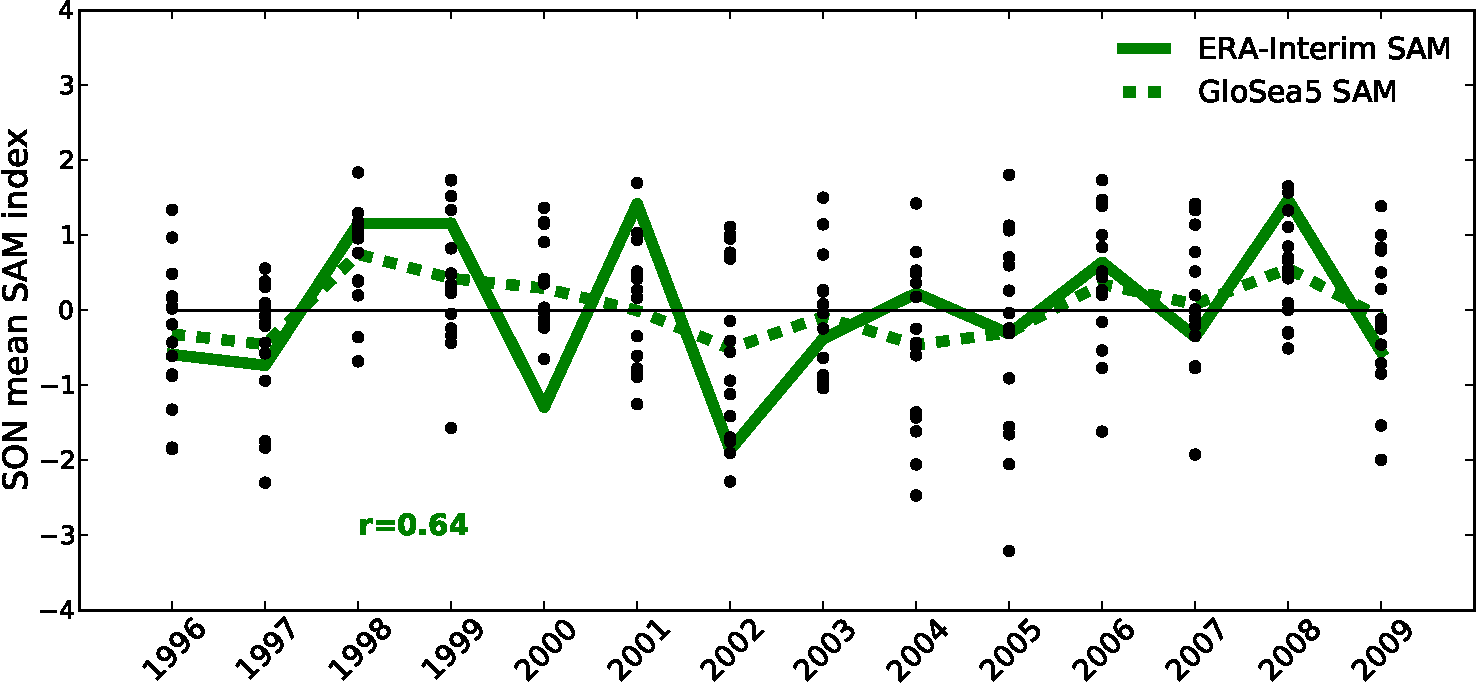
\includegraphics[width=\textwidth,angle=0]{figures/chapter-seasonal/sam_crop.pdf}\\
  \caption[GloSea5 predictions of the SAM.]{SON mean Southern Annular Mode (SAM)
index in individual GloSea5 hindcast ensemble members (dots), ensemble mean
(dashed green curve) and ERA-Interim (solid green curve). The SAM is calculated
from mean sea-level pressure data, and hindcasts initialised near 1st
August. The correlation of the ensemble mean and ERA-Interim values is 0.64,
which is statistically significant at the 99\% level.}\label{fig:sam_ts}
\end{figure}

Figure \ref{fig:mslp_tsrf_map}(a) shows the correlation of ERA-Interim and
GloSea5 SON averaged mean sea-level pressure anomalies at each grid point in the
Southern Hemisphere. As would be expected from the low frequency variability of
ENSO, correlations are greatest over the tropical Pacific. However, the
correlations are also as high as 0.7 across southern Australia and parts of
Antarctica.  On the other hand, correlations over southern Africa and South
America are not found to be significant. It is perhaps unsurprising that there
is little skill over the Andes region, since this is significantly above
sea-level, so mean sea-level pressure is not well defined.

\begin{figure}[t]
  \noindent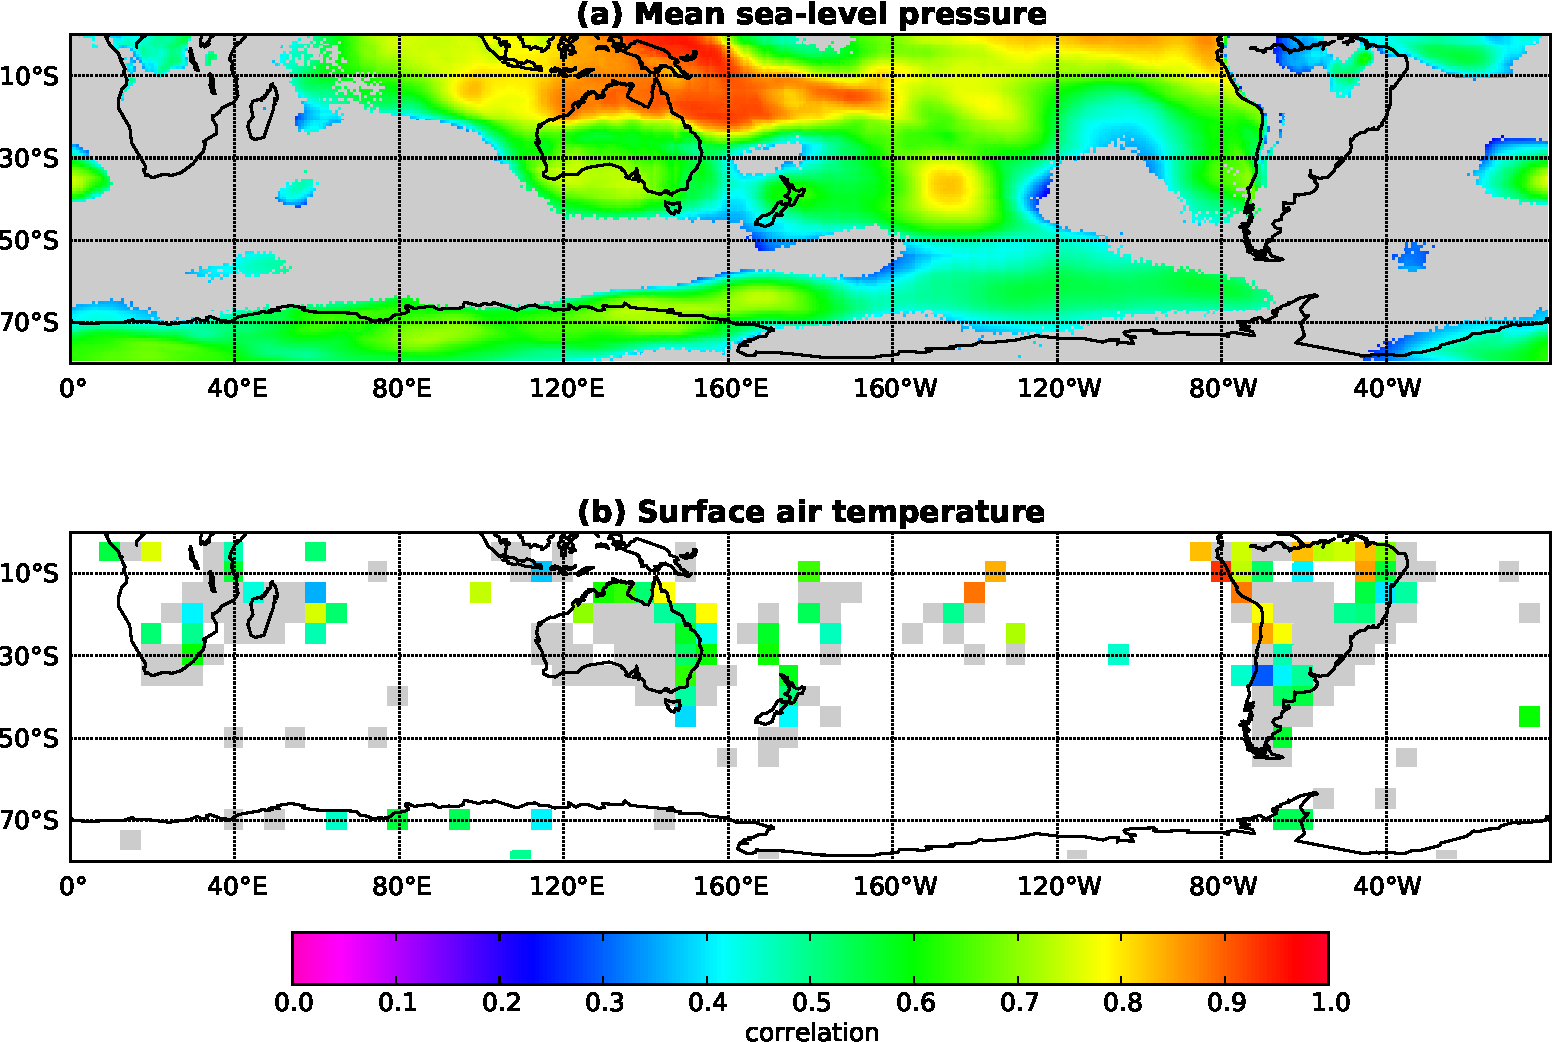
\includegraphics[width=\textwidth,angle=0]{figures/chapter-seasonal/mslp_tsrf_maps_crop.pdf}\\
  \caption[Correlation of GloSea5 forecasts of sea-level pressure and
temperature.]{(a) Correlation of SON mean sea-level pressure in the GloSea5
ensemble mean with ERA-Interim values. (b) Correlation of SON mean near-surface
air temperature in the GloSea5 ensemble mean and HadCRUT4 gridded station-based
temperature data. Regions with no observations are white and grey shading
indicates regions where the correlation is not greater than zero at the 95\%
confidence level, using a bootstrap test at each gridpoint.}\label{fig:mslp_tsrf_map}
\end{figure}

Correlations of GloSea5 SON average near-surface temperature with the gridded
station-based data set HadCRUT4 \citep{Morice2012} are shown in Fig.\
\ref{fig:mslp_tsrf_map}(b). This dataset is chosen because of the scarcity of
temperature observations in the Southern Hemisphere, which introduces
significant biases into reanalysis data. Again, the highest correlations are
found near the tropical Pacific, but significant correlations of about 0.5 are
found across eastern Australia, New Zealand and Antarctica. There are also
significant correlations in southern Africa and South America. The extratropical
regions where the greatest forecast skill is found are similar to those which
are observed to be most affected by variations in the SAM \citep{Gillett2006}.


\subsection{Stratosphere-troposphere coupling}

Given that statistically significant skill in hindcasts of the stratospheric
polar vortex is found at the same time of year as skill in predictions of the
SAM, the question arises as to whether skill in one may affect the other. In
order to investigate this, forecast skill as a function of lead-time and height
is studied for polar cap (60-90$^{\circ}$S) mean geopotential height anomalies
($Z'$)\footnote{At 1000~hPa monthly mean $Z'$ is highly correlated ($r=0.98$)
  with the SAM index}. Figure \ref{fig:gph_lag_corr}(a) shows the correlation of
$Z'$ in ERA-Interim with the GloSea5 ensemble mean hindcast values. Values are
smoothed with a 30-day running mean before correlations are calculated, and
plotted such that values for 15th September represent the correlation of the
ERA-Interim and GloSea5 ensemble mean September mean values (without this
smoothing, there are noisier but still significant correlations in a similar
pattern).

\begin{figure}[t]
  \noindent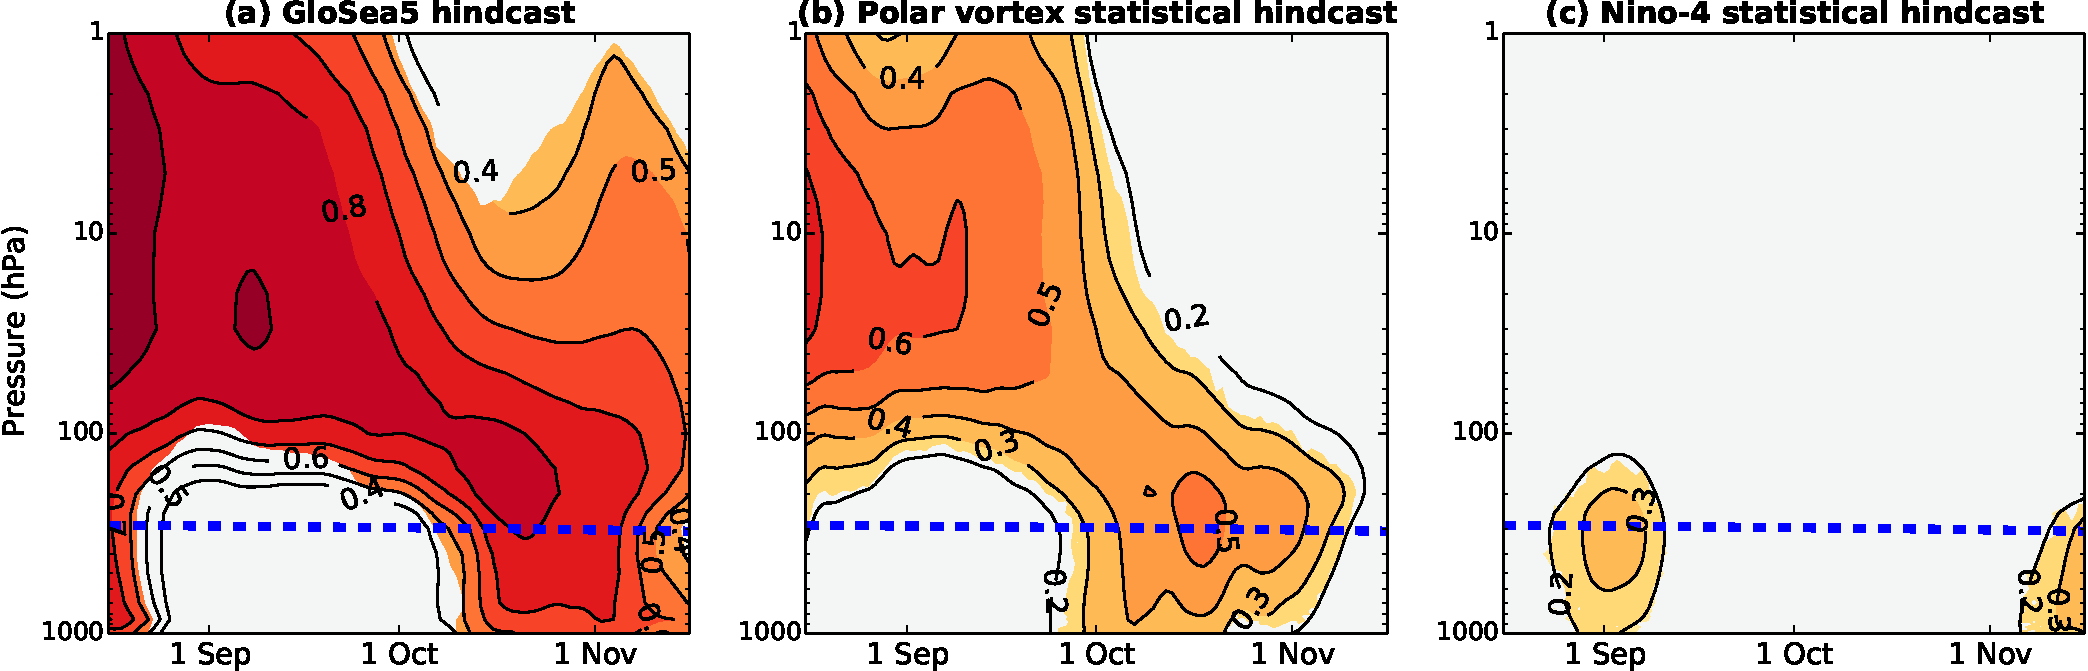
\includegraphics[width=\textwidth,angle=0]{figures/chapter-seasonal/lag_corr_crop.pdf}\\
  \caption[Lag-height correlation of GloSea5 polar cap geopotential height]{(a)
Correlation of GloSea5 ensemble mean polar cap (60-90$^{\circ}$S) geopotential
height anomalies ($Z'$) with ERA-Interim values from 1996--2009, as a function
of time and height. (b) Correlation of ERA-Interim from 1979--2010 values with
those predicted by a linear statistical model based on $Z'$ at 10~hPa on 1st
August. All values are smoothed with a 30-day running mean before correlations
are calculated. The contour interval is 0.1 and all colored regions are greater
than zero at the 95\% confidence interval, using a bootstrap test at each time
at height. The blue dashed line indicates the approximate polar cap mean
tropopause level \citep{Wilcox2012}.} \label{fig:gph_lag_corr}
\end{figure}

As would be expected from the initialisation of GloSea5 from ERA-Interim data,
correlations are high in both the troposphere and the stratosphere for the
August mean, due to predictability on weather timescales. However, tropospheric
and lower-stratospheric skill rapidly decays and becomes statistically
insignificant throughout September. In contrast, stratospheric correlations
remain statistically significant throughout the hindcast simulation, and as high
as 0.8 through to mid-October (corresponding to a 2--3 month lead time). This
observed greater stratospheric than tropospheric skill might be expected from
the longer `memory' of the stratosphere; SAM decorrelation timescales are about
60--70 days in the stratosphere but only about 10 days in the troposphere during
SON \citep{Simpson2011}.

Importantly, the region of high levels of stratospheric skill descends with time
and is present at the tropopause at the same time as a re-emergence of
significant tropospheric skill in mid-October. This re-emergence cannot be
accounted for by the persistence of tropospheric anomalies, so must be the
result of the effect of another predictable signal on the tropospheric
circulation. An obvious candidate for such a signal is the polar stratosphere,
since this remains predictable throughout the hindcast period. The re-emergence
of tropospheric skill also occurs at the same time as the strongest observed
coupling between the stratosphere and troposphere found in other studies
\citep[e.g.,][]{Thompson2005, Simpson2011}.

In order to determine the stratospheric influence on tropospheric skill, a
simple statistical forecast model is formed, which has as its only input the
initial conditions of the Antarctic stratosphere. ERA-Interim values are used to
produce this model based on the linear regression of $Z'$ at 10~hPa on 1st
August with $Z'$ at all other times and heights for 31 of the 32 years from
1979--2009. This model is then used to produce a hindcast of the 32nd year based
on its $Z'$ at 10~hPa on 1st August. The method ensures that no information from
the hindcast year enters the model. The process is then repeated to make
hindcasts of all 32 years; a procedure known as leave-one-out cross validation
\citep{Wilks}.

Figure \ref{fig:gph_lag_corr}(b) shows the average correlation of 30-day running
means of these statistical forecasts with ERA-Interim values. As might be
expected, skill is initially high in the mid-stratosphere but not the
troposphere. As with the GloSea5 hindcasts, the region of high skill descends
with time, and statistically significant correlations re-emerge in the
troposphere throughout October. This demonstrates that skilful forecasts of the
Antarctic troposphere during October can be produced based only on knowledge of
$Z'$ in the mid-stratosphere on 1st August. It also suggests that the
re-emergence of tropospheric skill in the GloSea5 hindcasts in October is likely
to be caused by persistent stratospheric anomalies which descend with time.

The statistical hindcasts in Fig.\ \ref{fig:gph_lag_corr}(b) show lower skill
than the GloSea5 hindcasts at all times, and do not show statistically
significant tropospheric correlations, nor the increase in upper-stratospheric
skill during November. These observations could potentially be explained by the
importance of non-linearities or the influence of external factors, such as
ENSO, on the Antarctic stratosphere-troposphere system. Indeed, statistical
hindcasts similar to those shown in Fig.\ \ref{fig:gph_lag_corr}(b) were
produced based on the Ni\~no-3 index, and found to have statistically
significant tropospheric skill during November, but none at other times or
heights. This is consistent with the results of \citet{Lim2013}, who find the
greatest correlation between tropical Pacific sea-surface temperatures and the
SAM during November--January.

\section{Discussion}

We have demonstrated that Antarctic total column ozone amounts are predictable
up to four months in advance during the austral spring, even with a model which
lacks interactive chemistry. While using such a model has the advantage of being
less computationally expensive than a chemistry-climate model, there are also
some drawbacks. Primarily, the model will not be able to simulate zonal
asymmetries in ozone concentrations or the feedback between ozone concentrations
and stratospheric temperatures. Both these factors have been shown to be
important in driving long-term trends in the SAM as a result of ozone depletion
\citep{Thompson2002a, Crook2008, Waugh2009}.

Perhaps more relevant for seasonal forecasts is the fact that we have not been
able to determine whether the observed strong correlation between the
stratospheric circulation and Antarctic ozone concentrations is dominated by a
chemical or dynamical mechanism. If the relationship is dominated by a chemical
mechanism, whereby enhanced descent over the pole inhibits the activation of
ozone-depleting substances, we would expect the correlation to weaken as
concentrations of these substances return to pre-industrial levels. Accurate
forecasts of ozone with models lacking interactive chemistry would then not be
possible. On the other hand, if the mechanism is largely dynamical, whereby
transport of ozone-rich air from the tropics is the important factor, we would
not expect the relationship to change in time.  Although a study to distinguish
these mechanisms has been carried out for chemistry-climate models
\citep{Garny2011}, it has not been possible to do so in observations. In either
case, we do not expect the relationship to break down soon, as concentrations of
ozone-depleting substances are not projected to return to 1980 levels until the
late 21st century \citep{WMO2010}.

The correlation skill of 0.64 for the SON mean SAM in the GloSea5 hindcasts is
greater than that of other contemporary seasonal forecast systems at similar
lead times. For instance, \citet{Lim2013} report a correlation of 0.3--0.4 for
the SON mean SAM from 1st August initialised forecasts using the Predictive
Ocean and Atmosphere Model for Australia, version 2 (POAMA2). Significantly,
this system has only two model levels in the stratosphere, and so is unable to
simulate the stratosphere-troposphere coupling described here. \citet{Lim2013}
suggest that the significant SAM predictability found from October--January in
their system is the result of the influence of ENSO through a tropospheric
teleconnection.  These findings are not inconsistent with our results, since
this time period is beyond the extent of the GloSea5 hindcasts, and largely
after the stratospheric final warming, when the stratosphere is much less
variable. \citet{Lim2013} were also mostly concerned with longer range forecasts
(up to 6-month lead time) which are beyond the persistence time scales of the
Antarctic stratosphere, but within those of the tropical Pacific.

Despite this significant correlation skill in hindcasts of the SAM, it is clear
from \ref{fig:sam_ts} that the amplitude of the ensemble mean hindcast is much
less than that of observations. The signal-to-noise ratio (ratio of the standard
deviation of the ensemble mean to that of all ensemble members) is just 0.4. For
a `perfect' forecast system (one in which observations are indistinguishable
from an ensemble member), the signal-to-noise ratio and correlation are directly
related \citep{Kumar2009}, so that the expected correlation would be just
0.3. The fact that it is greater than this is because the average correlation
between ensemble members and observations is much greater than that between
pairs of ensemble members. A similar but smaller difference is also found for
the stratospheric polar vortex forecasts. These results mean that individual
ensemble members have a smaller predictable signal than observations.

Given this result, it might be expected that more skillful predictions could be
obtained with a larger ensemble size. To illustrate the variation of hindcast
skill with ensemble size we systematically sample smaller sets of forecasts from
the full 15 members for each year, following the method of
\citet{Scaife2013}. This is repeated many times and an average value for a given
sample size calculated. This variation of correlation skill with ensemble size
for both the SON mean SAM and stratospheric polar vortex winds is shown in Fig.\
\ref{fig:corr_ens_size_sh}. These curves closely follow the theoretical
relationship of \citet{Murphy1990}, which relies only on the mean correlation
between pairs of ensemble members, $\langle r_{mm} \rangle$, and the mean
correlation between individual ensemble members and observations,
$\langle r_{mo} \rangle$, given by
\begin{equation} r = \frac{\langle r_{mo} \rangle \sqrt{n}}{\sqrt{1+(n-1)\langle
r_{mm} \rangle}}
\end{equation} where $r$ is the ensemble mean correlation, and $n$ is the
ensemble size. These curves are shown in Fig.\ \ref{fig:corr_ens_size_sh}, along
with their asymptote for an infinite sized ensemble. Although the stratospheric forecasts
cannot be greatly improved with a larger ensemble size in the current system,
correlation scores of about 0.7 of the SAM could be achieved with an ensemble
size near 30. Both have an asymptote near 0.8, similar to that found by
\citet{Scaife2013} for the NAO.

\begin{figure}[t]
  \centering
  \noindent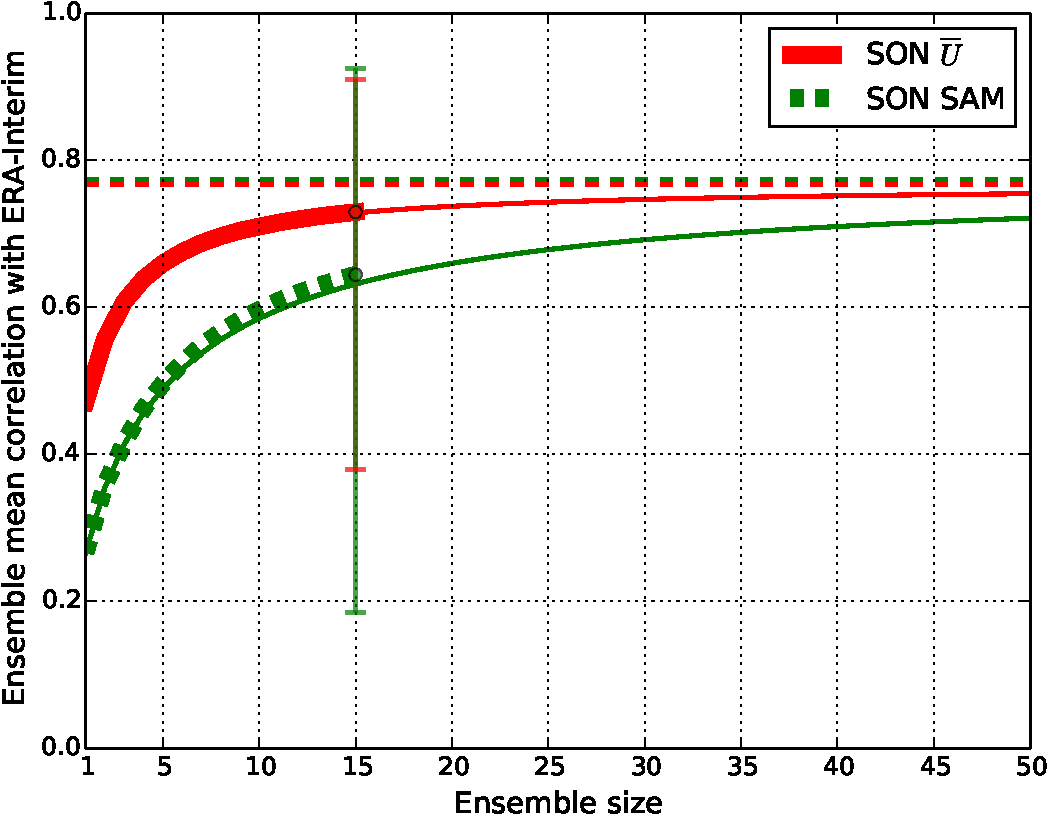
\includegraphics[width=0.6\textwidth,angle=0]{figures/chapter-seasonal/corr_ens_size_crop.pdf}\\
  \caption[Variation of GloSea5 forecast skill with ensemble size]{GloSea5
ensemble mean correlation with ERA-Interim as a function of ensemble size for
the SON mean $\overline{U}$ at 10~hPa and 60$^{\circ}$S and SON mean SAM (thick
lines). A theoretical estimate of the variation of correlation with ensemble
size is shown in each case (thin solid lines), along with its asymptote for an
infinite sized ensemble (dashed lines)}\label{fig:corr_ens_size_sh}
\end{figure}


\section{Conclusions}

Using a set of seasonal hindcasts initialised at the start of the austral
spring, we have demonstrated skillful prediction of the interannual variability
of the Antarctic stratospheric polar vortex at 1-4 month lead times. This
includes extreme events such as the 2002 SSW, which is the most extreme year in
the ensemble mean, and has one ensemble member which simulates a SSW. Because
this variability is observed to be closely correlated with Antarctic column
ozone amounts, we are able to infer skillful prediction of interannual
variability in Antarctic ozone depletion.

We also find significant skill, which exceeds that of other contemporary
seasonal forecast systems, in hindcasts of the spring mean SAM index.  By
studying the variation of this skill with time and height, we suggest that this
skill is influenced by stratospheric anomalies which descend with time and are
coupled with the troposphere in October and November. In fact, the influence of
the stratosphere is such that skillful statistical predictions of the October
SAM can be made using only information from 1st August in the mid-stratosphere.

Assuming that the 14 year period studied here is representative of future years,
these results suggest that it may now be possible to make skillful seasonal
forecasts of interannual variations in ozone depletion and large scale weather
patterns across the Southern Hemisphere. They also demonstrate the importance of
the inclusion of a well-resolved stratosphere in seasonal forecast models.

 \begin{figure}[p] \vspace*{-3cm} \centering
 \noindent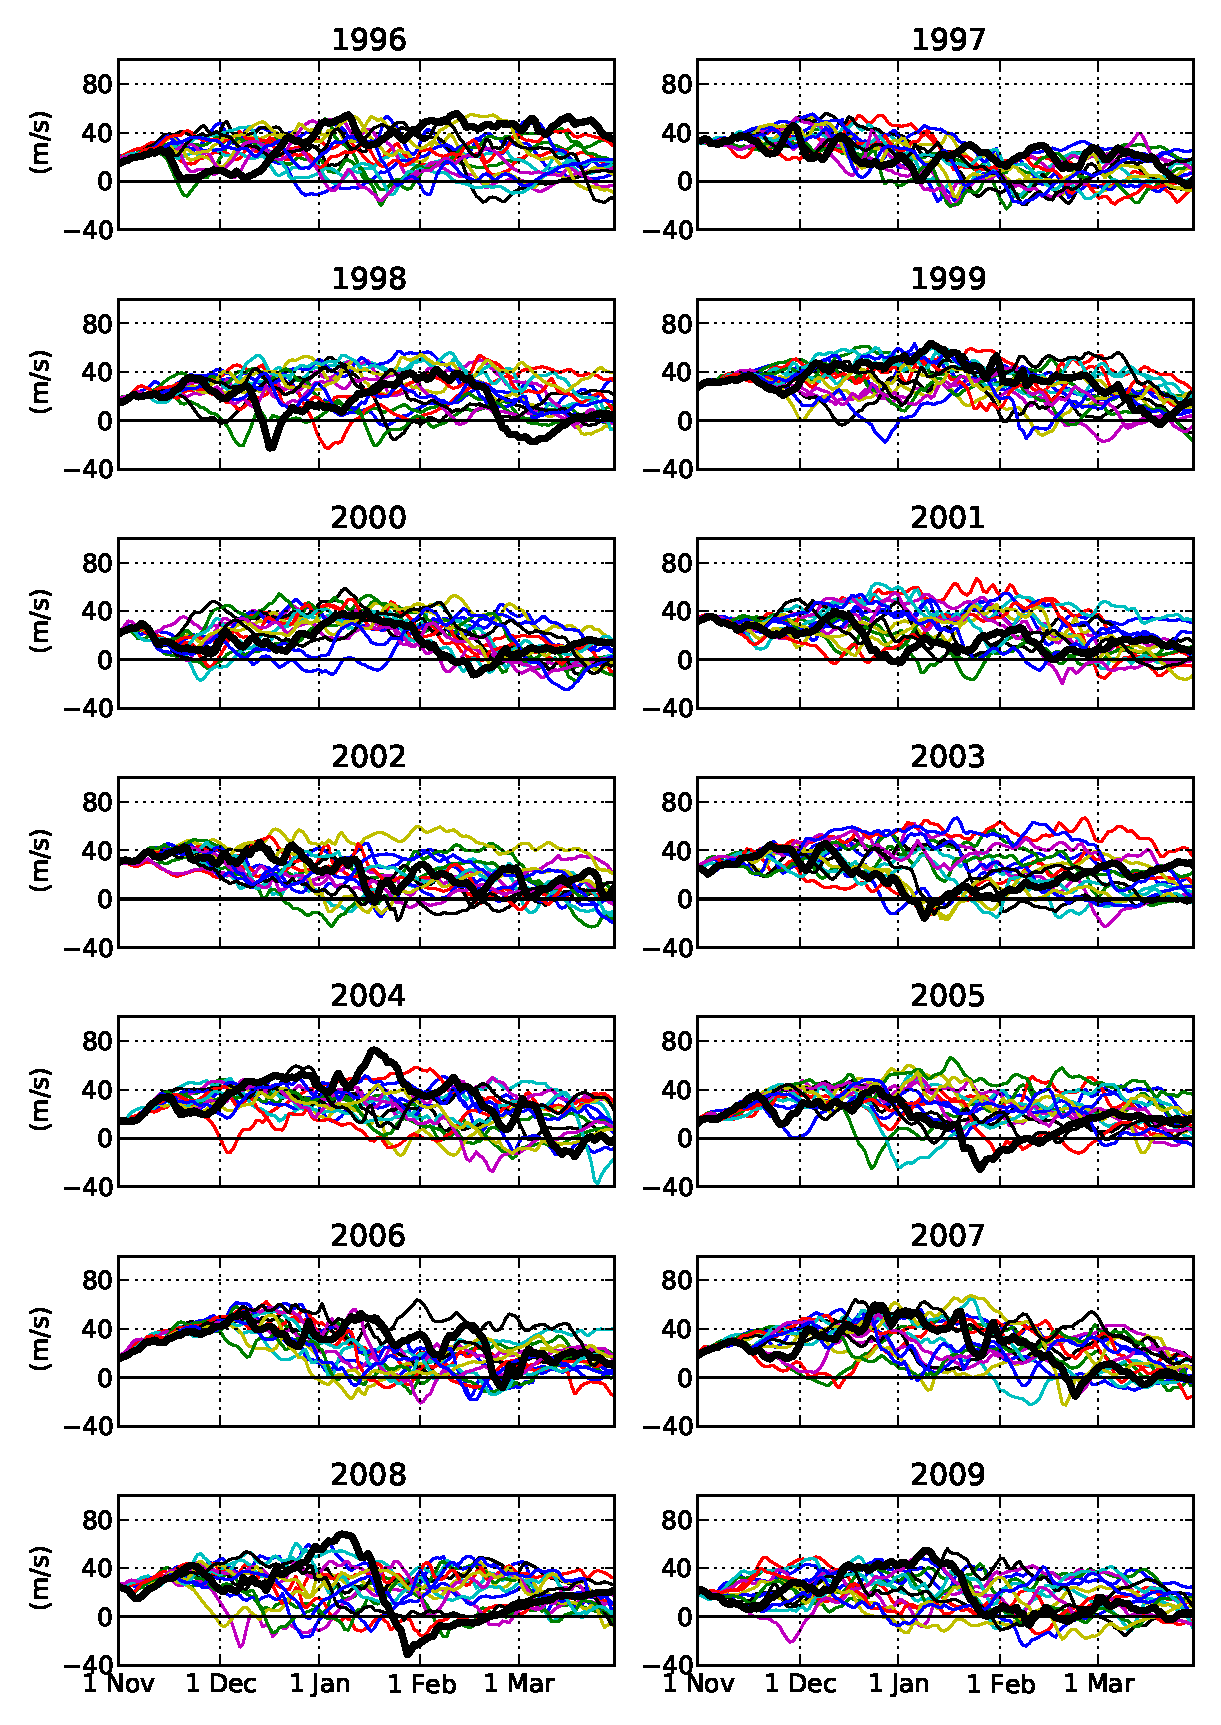
\includegraphics[width=40pc]{figures/chapter-seasonal/zm_winds_nh_poststamp.pdf}
 \caption[Timeseries of $\overline{U}$ at 60$^{\circ}$N, 10~hPa, for all GloSea5
ensemble members.]{Timeseries of zonal-mean zonal wind in the Arctic polar
vortex ($60^{\circ}$N, 10~hPa) in the ERA-Interim reanalysis (thick black lines)
and the GloSea5 ensemble hindcasts (thin coloured lines). Individual ensemble
members are initialised from dates centred on November 1st. }
 \label{fig:nh_poststamp}
 \end{figure}

 \begin{figure}[p] \vspace*{-3cm} \centering
 \noindent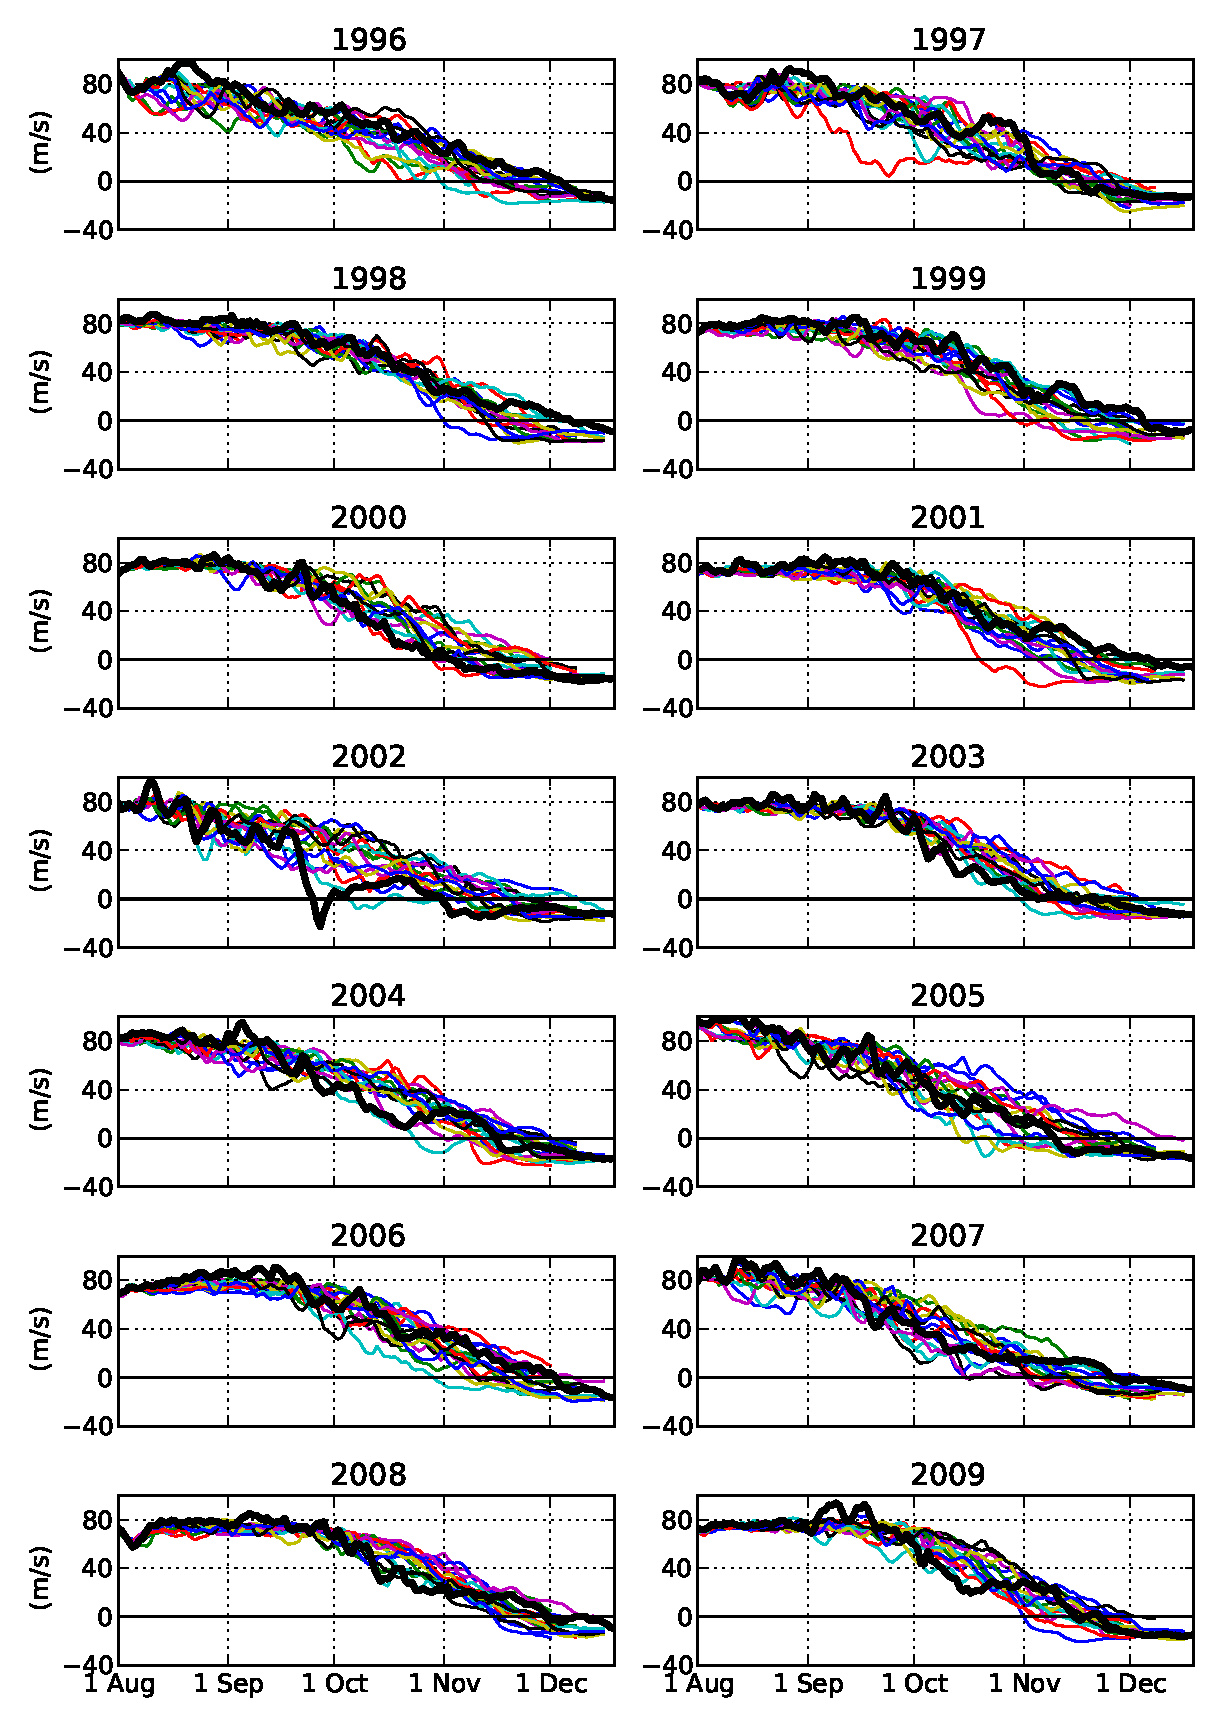
\includegraphics[width=40pc]{figures/chapter-seasonal/zm_winds_sh_poststamp.pdf}
 \caption[Timeseries of $\overline{U}$ at 60$^{\circ}$S, 10~hPa, for all GloSea5
ensemble members.]{As figure \ref{fig:nh_poststamp} but for the zonal-mean zonal
wind in the Antarctic polar vortex ($60^{\circ}$S, 10~hPa), and ensemble members
initialised from dates centred on August 1st.}
 \label{fig:sh_poststamp}
 \end{figure}

 \begin{figure}[p] \vspace*{-3cm} \centering
 \noindent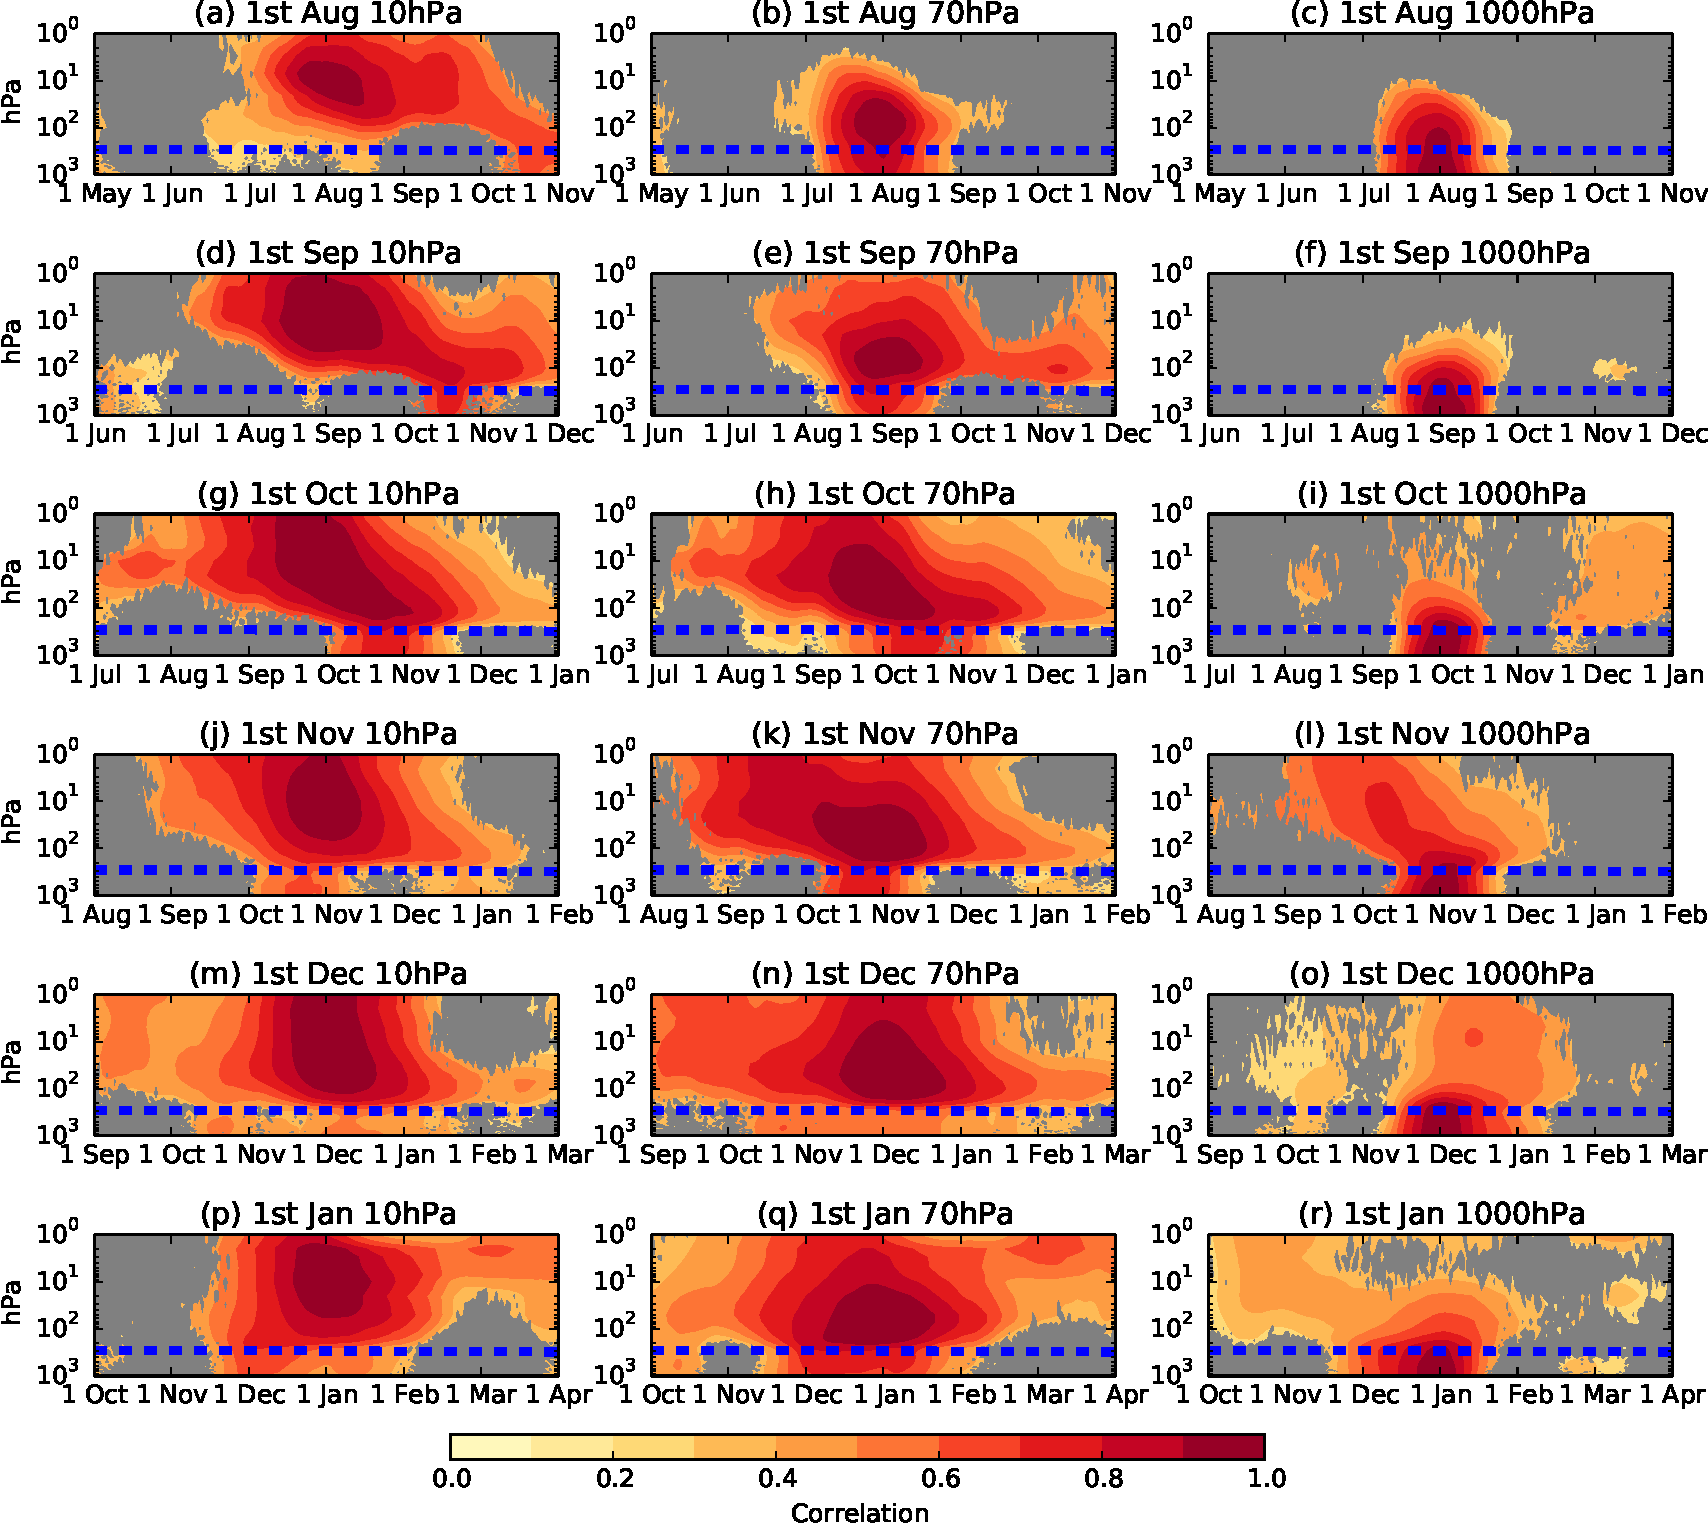
\includegraphics[width=\textwidth]{figures/chapter-seasonal/lag_height_corr_obs.pdf}
 \caption[Lag-height correlation of $Z'$ at 10~hPa and 1000~hPa.]{Correlation of
   ERA-Interim (1979--2010) Z' at 10~hPa, 70~hPa, and 1000~hPa with Z' at other
   times and lags. Values are smoothed with a 30-day running mean before
   correlations are calculated, and colours represent correlations that are 95\%
   significant from zero according to a bootstrap test.}
 \label{fig:lag_height_corr_obs}
 \end{figure}

\begin{figure}[t]
  \noindent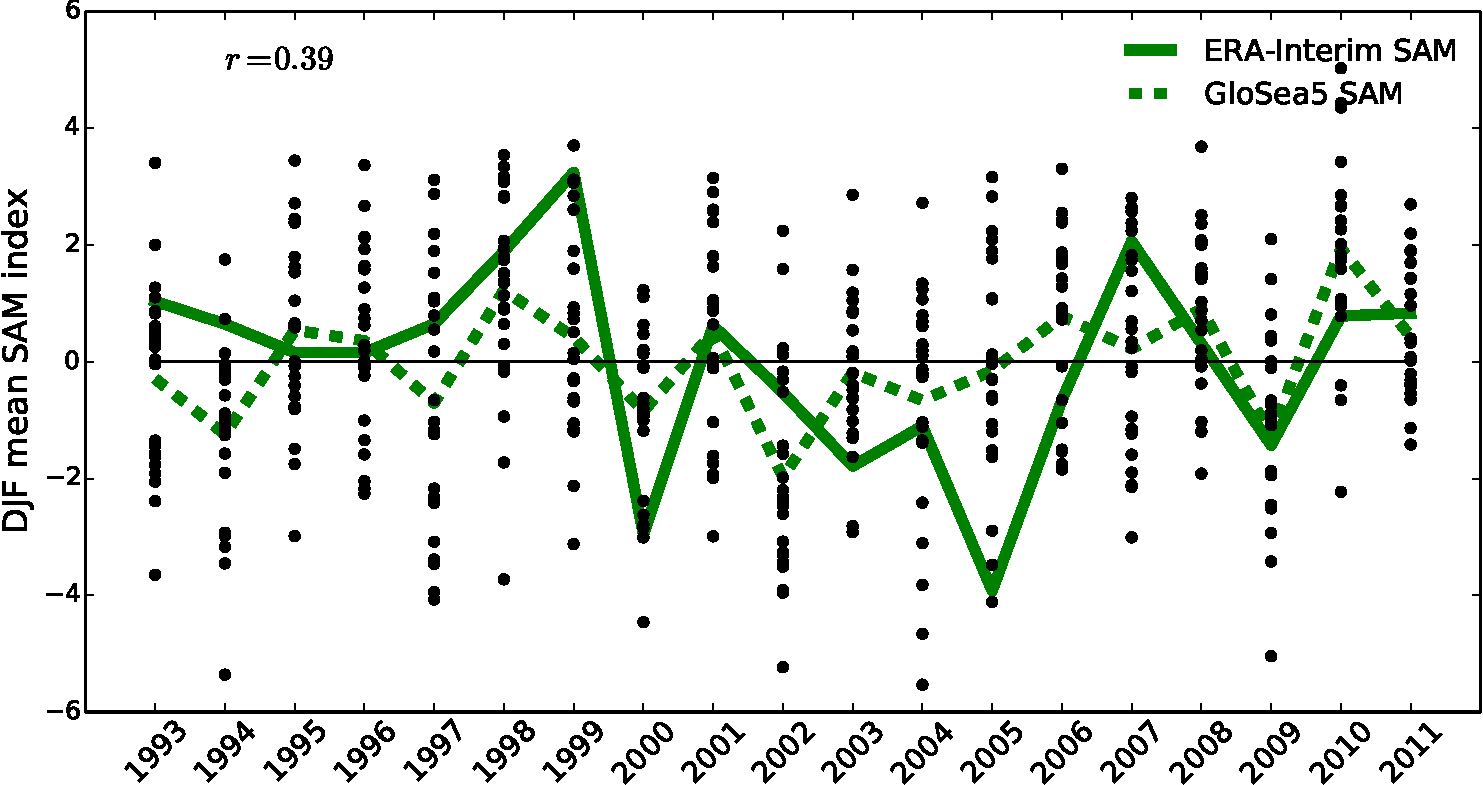
\includegraphics[width=\textwidth,angle=0]{figures/chapter-seasonal/DJF_SAM.pdf}\\
  \caption[GloSea5 predictions of the SAM.]{DJF mean Southern Annular Mode (SAM)
    index in individual GloSea5 hindcast ensemble members (dots), ensemble mean
    (dashed green curve) and ERA-Interim (solid green curve). The SAM is
    calculated from mean sea-level pressure data, and hindcasts initialised near
    1st November. The correlation of the ensemble mean and ERA-Interim values is
    0.39}\label{fig:djf_sam_ts}
\end{figure}


\begin{subappendices}
\section{Choice of time period for statistical forecast}

\begin{figure}[t]
  \noindent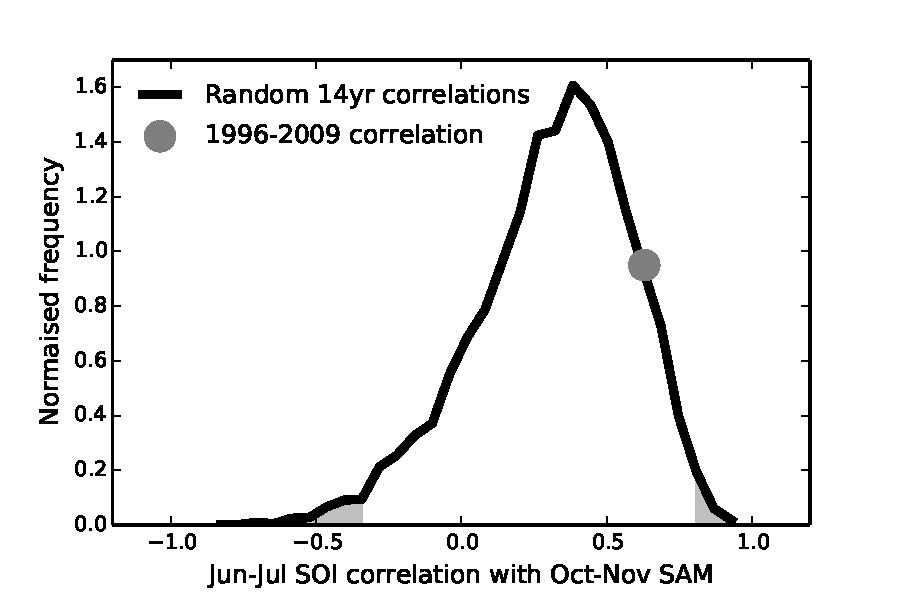
\includegraphics[width=0.7\textwidth,angle=0]{figures/chapter-seasonal/SAM_SOI_corr.pdf}\\
  \caption[Correlation of the SOI with the SAM.]{Histogram of correlations of
    random 14-year samples of detrended June-July SOI with October-November
    SAM. Also shown is the correlation over the 1996--2009 hindcast period. Grey
  shading indicates the $<2.5$\% and $>97.5$\% ranges.}\label{fig:sam_soi_corr}
\end{figure}

\begin{figure}[t]
  \noindent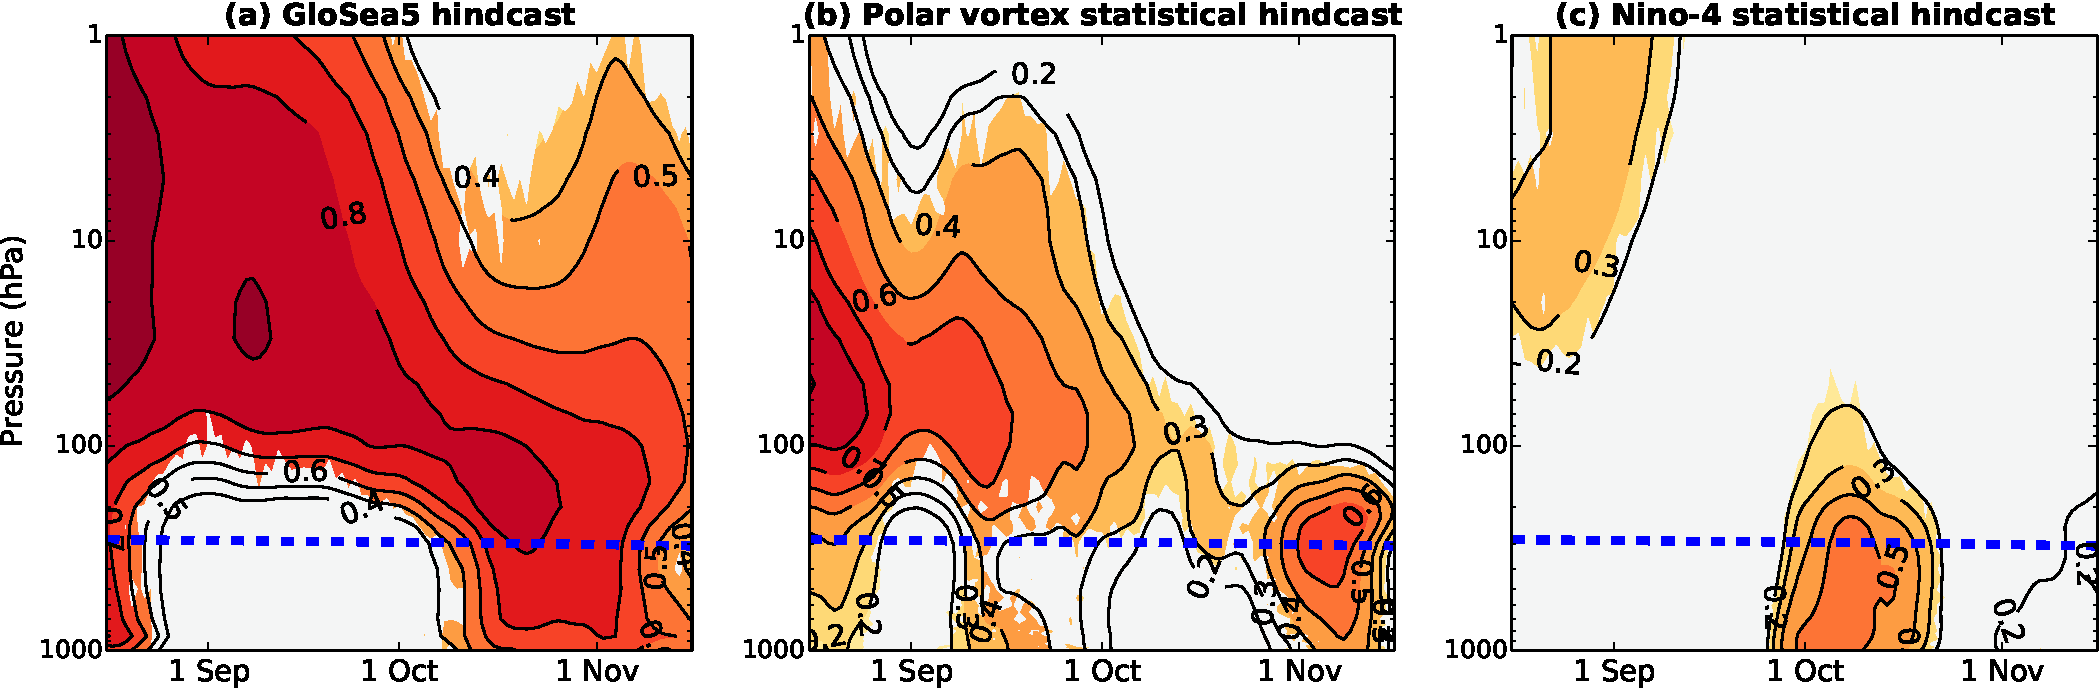
\includegraphics[width=\textwidth,angle=0]{figures/chapter-seasonal/lag_height_short.pdf}\\
  \caption[Lag-height correlation of GloSea5 polar cap geopotential height]{As
    Figure \ref{fig:gph_lag_corr} but all analysis restricted to the 1996--2009
    period.}\label{fig:lag_height_short}
\end{figure}

\end{subappendices}


%%% Local Variables:
%%% mode: latex
%%% TeX-master: "thesis"
%%% End:
